
\documentclass[12pt, a4paper]{uhthesis}


\usepackage[T1]{fontenc}

\usepackage[utf8]{inputenc}
\usepackage[spanish]{babel}
%\decimalpoint

%\usepackage{subfigure}
\usepackage[linesnumbered,lined,titlenumbered,ruled]{algorithm2e}
\usepackage{amsmath}
\usepackage{amssymb}
\usepackage{amsbsy}
\usepackage{mathpazo}
\usepackage{float}
\usepackage{graphicx}

\usepackage{amsfonts}
\usepackage{amsmath}
\usepackage{amsthm}
\usepackage{fancyhdr}
\usepackage{subcaption}
%\usepackage{graphicx, setspace}
\usepackage{caption}
%\captionsetup[figure]{font={stretch=1.2}}


\usepackage{hyperref}

\usepackage[scaled]{beramono}
\usepackage{color}
\usepackage{listings}

\usepackage{graphicx}
\usepackage{float}
\usepackage{array}
\newcolumntype{P}[1]{>{\centering\arraybackslash}p{#1}}
\newcolumntype{M}[1]{>{\centering\arraybackslash}m{#1}}

\usepackage[flushleft]{threeparttable}

\renewcommand{\tablename}{Tabla}

\title{Dise\~no de un protocolo para la medici\'on de la actividad de enzimas de defensa en plantas de \textit{Raphanus sativus}.} %\linebreak de La Habana, Cuba}
\author{ Sheila Toledo Blanco } 
\advisor{Dr. Georgina Espinosa L\'opez\\Lic. Elaine Puentes Berm\'udez }
\faculty{Facultad de Biología}
\date{Septiembre de 2020}
\logo{Graphics/uhlogo}
\makenomenclature

\renewcommand{\vec}[1]{\boldsymbol{#1}}
\newcommand{\diff}[1]{\ensuremath{\mathrm{d}#1}}

\usepackage[
top=30mm,
bottom=30mm,
left=25mm,
right=25mm
]{geometry}

%\setlength{\parindent}{10cm}

\usepackage{natbib}
\usepackage{hyperref}
\newcommand*{\urlprefix}{Disponible en: }
\newcommand*{\urldateprefix}{Visitado } 

\usepackage{chngcntr}
\counterwithout{figure}{chapter}
\counterwithout{table}{chapter}

\linespread{1.44}\selectfont

\begin{document}

\frontmatter

\maketitle


\

\vspace{20cm}

\begin{flushright}
\it A ustedes, que son mis pilares.
\end{flushright}
\



{\it{\bf \Huge Agradecimientos }}

\vspace{1.3cm}


\medskip
\medskip
\medskip

A mis tutoras Georgina Espinosa y Elaine Puentes quienes me han guiado en este camino, brind\'andome sus conocimientos y apoy\'andome en cada paso. Gracias por transmitirme su experiencia, por ser mis ejemplos e influir tanto en mi formaci\'on. Sin ustedes este trabajo no hubiese sido posible. A ambas, infinitas gracias. 

\medskip
\medskip
\medskip

A todos los profesores de la Facultad de Biología, quiénes fueron esenciales en mi formaci\'on profesional. A mis compañeros de la universidad y amigos, a Katherine Men\'endez, Ana Jessica D\'iaz, y en especial a Isabel L\'opez, por su apoyo imprescindible. 

\medskip
\medskip
\medskip

Por último y no menos importante a mi familia, mi abuela, mi t\'io y mis padres quienes han sido esenciales en mi formaci\'on, sin ustedes esto no fuese posible. A mis segundos padres, mis trikis, gracias por su cari\~no, por hacerme crecer cada d\'ia. \\

En especial, a Albe, gracias por ser un pilar fundamental en toda esta experiencia y darme fuerzas cuando m\'as lo necesitaba. 






\medskip
\medskip
\medskip
\medskip
\medskip
\medskip
\medskip
\medskip
\medskip
\medskip
\medskip
\medskip
\medskip
\medskip
\medskip
\begin{flushright}
A todos sinceramente, \emph{Muchísimas Gracias}. 
\end{flushright}
\clearpage
\section*{Listado de abreviaturas y acrónimos}

\begin{description}
\item[AS:] \'Acido salic\'ilico.
\item[BL:] Brasin\'olida.
\item[BRI1:] \textit{Receptor Brassinosteroid-Insentive 1}.
\item[BRs:] Brasinoesteroides.
\item[BSA:] Albúmina de Suero Bovino, \textit{Bovine albumin serum} (por sus siglas en inglés).	
\item[CAT:] Catalasa.
\item[CBBG:] Azul Coomassie Brillante G-250, \textit{Coomassie Brilliant Blue G-250} (por sus siglas en inglés).
\item[CNPR:] Centro de Investigación de Productos Naturales.
\item[DETAPAC:] \textit{Diethylene Triamine Penta Acetic Acid} (por sus siglas en inglés)
\item[EDTA:] \textit{ Ethylene Diamine Tetraacetic Acid} (por sus siglas en inglés). 
\item[ETI:] Inmunidad Desencadenada por Efectores, \textit{Effector-Triggered Immunity} (por sus siglas en inglés).
\item[EtOH:] Etanol.
\item[HR:] Respuesta Hipersensible, \textit{Hypersensitive Response} (por sus siglas en inglés).
\item[L-DOPA:] L-dihidroxifenilalanina, \textit{L-dihydroxy phenylalanine} (por sus siglas en inglés).
\item[LRR:] Repeticiones Ricas en Leucina, \textit{Leucine rich repeat} (por sus siglas en ingl\'es). 
\item[NaCl:] Cloruro de Sodio.
\item[DO]: Densidad \'optica.
\item[PAMP/MAMPs:] Patrones Moleculares Asociados a Patógenos, \textit{Pathogenor Microbe-Associated Molecular Patterns} (por sus siglas en inglés).
\item[PPO:] Polifenol oxidasa, \textit{Polyphenol oxidase} (por sus siglas en inglés).
\item[PRRs:] Receptores de Reconocimiento de Patrones, \textit{Pattern Recognition Receptors} (por sus siglas en inglés).
\item[PTI:] Inmunidad Desencadenada por Patrones, \textit{Pattern Triggered Immunity} (por sus siglas en inglés).
\item[PUFA:] \'Acidos grasos poli-insaturados, \textit{polyunsaturated fatty acid} (por sus siglas en inglés).
\item[PVPP:] Polivinil Pirrolidona.
\item[ROS:] Especies reactivas del ox\'igeno, \textit{reactive oxygen species} (por sus siglas en inglés). 
\item[SOD:] Super\'oxido dismutasa.
\item[24-epiBL:] 24-epibrasin\'olida.
\item[28-HomoBL:] 28-homobrasin\'olida.








\end{description}

{\bf \LARGE Resumen}

\medskip
\medskip
\medskip
\medskip
\medskip
\medskip

Las plantas son organismos sésiles que se enfrentan a condiciones adversas tanto bióticas, como abióticas. Ante estas condiciones se desencadenan respuestas de defensa que incluyen el aumento de la actividad de un grupo de enzimas. Los diferentes mecanismos de defensa son regulados mediante fitohormonas, entre ellas los brasinoesteroides (BRs), cuya aplicación exógena o la modificación de su contenido en plantas, puede conducir al incremento de la actividad de estas enzimas. Este trabajo tiene como objetivo diseñar un protocolo que permita la posterior evaluación del efecto de dos análogos sintéticos de BRs en las enzimas de defensa superóxido dismutasa (SOD), catalasa (CAT) y polifenol oxidasa (PPO) en plantas de \textit{Raphanus sativus}. En el trabajo se identifican las metodologías para la preparación de extractos enzimáticos que permitan evaluar la actividad de las mismas. Para la medición de SOD se establece la metodología de extracción con acetona como correcta, mientras que las enzimas CAT y PPO se evalúan en extractos acuosos. Se establecen los ensayos que permiten la determinación de los parámetros cinéticos de las enzimas SOD, CAT y PPO en extractos enzimáticos crudos.


\medskip
\medskip
\medskip
\medskip
\medskip
\medskip
\medskip
\medskip
\medskip
\medskip
\medskip
\medskip
\medskip
\medskip

{\bf Palabras clave:} catalasa,  extractos enzim\'aticos crudos, polifenol oxidasa, \textit{Raphanus sativus}, super\'oxido dismutasa.



{\bf \LARGE Abstract}

\medskip
\medskip
\medskip
\medskip
\medskip
\medskip

Plants are sessile organisms that face adverse conditions, both biotic and abiotic. These conditions trigger defensive responses that include increased activity of a group of enzymes. The different defense mechanisms are regulated by phytohormones, among them brassinosteroids (BRs), whose exogenous application or the modification of their content in plants can lead to an increase in the activity of these enzymes. This work aims to design a protocol that allows the subsequent evaluation of the effect of two synthetic BRs analogues on the defense enzymes superoxide dismutase (SOD), catalase (CAT) and polyphenol oxidase (PPO) in \textit{Raphanus sativus} plants. The work identifies the methodologies for the preparation of enzyme extracts that allow evaluating their activity. For the measurement of SOD, the acetone extraction methodology is established as correct, while the CAT and PPO enzymes are evaluated in aqueous extracts. The tests that allow the determination of the kinetic parameters of the enzymes SOD, CAT and PPO in crude enzyme extracts are established.




\medskip
\medskip
\medskip
\medskip
\medskip
\medskip
\medskip
\medskip
\medskip
\medskip
\medskip
\medskip
\medskip 
\medskip

 {\bf Keywords:} catalase, enzymatic crude extract, polyphenol oxidase, \textit{Raphanus sativus}, superoxide dismutase.

\tableofcontents 
\addtocontents{toc}{\protect\thispagestyle{empty}}
\pagenumbering{gobble}
\clearpage

\mainmatter



\chapter*{Introducción}  
\addcontentsline{toc}{chapter}{Introducción}

Las plantas son productores primarios que desempe\~nan un papel fundamental en la sostenibilidad de la vida en la Tierra \citep{mithofer2016general} y representan una rica fuente de nutrientes para muchos organismos, incluyendo: bacterias, hongos, protistas, insectos y vertebrados. Por su parte, los hombres dependen casi exclusivamente de las plantas para la alimentaci\'on y las utilizan, adem\'as, para la obtenci\'on de otros productos importantes como maderas, medicinas y biocombustibles \citep{freeman2008overview}.\\

Las plantas son organismos s\'esiles, por lo que est\'an obligados a discriminar entre los diferentes retos que les plantea su entorno y responder a ellos \citep{vivanco2005mecanismos}. Continuamente se enfrentan a condiciones adversas tanto bióticas, como abióticas, frente a las cuales se desencadenan respuestas de defensa. \\

Entre los mecanismos de defensa que se pueden desencadenar se incluye el aumento de la actividad de enzimas que participan en las respuestas de defensa, como la super\'oxido dismutasa (SOD), la catalasa (CAT) y la polifenol oxidasa (PPO).\\

La SOD es una familia de enzimas que constituye la primera l\'inea de defensa antioxidante en plantas, catalizando la descomposici\'on de una de las especies reactivas del ox\'igeno (ROS, por sus siglas en ingl\'es), el ani\'on super\'oxido. La actividad de la enzima le permite a la planta mantener un balance entre la producci\'on y eliminaci\'on de este ani\'on, que a altas concentraciones puede provocar da\~nos significativos en las estructuras celulares \citep{gill2015superoxide}.\\
 
La CAT es una hemoprote\'ina tetram\'erica que est\'a presente en la mayor\'ia de los organismos aerobios y es una de las enzimas principales en el catabolismo del per\'oxido de hidr\'ogeno \citep{luhova2003activities}. El per\'oxido de hidr\'ogeno participa en numerosos procesos de regulaci\'on dentro de la planta \citep{xie2019roles} y su balance es imprescindible, ya que puede ocasionar da\~nos oxidativos a estructuras celulares. Adem\'as, a partir del per\'oxido de hidr\'ogeno, en presencia de metales de transici\'on, se puede formar el radical hidroxilo que tiene la capacidad de reaccionar rápidamente con todo tipo de macromoléculas y no existe un mecanismo enzimático que lo elimine \citep{moller2007oxidative}.  \\

La PPO son una familia de metaloenzimas monom\'ericas que reaccionan con una amplia gama de sustratos fen\'olicos, catalizando la oxidaci\'on de fenoles propios de la c\'elula a quinonas. Han sido implicadas en las respuestas de defensa de las plantas debido a la aparici\'on de sus productos de reacci\'on en el momento de ataques de pat\'ogenos e insectos, lesiones y diferentes tipos de estr\'es \citep{mayer1979polyphenol, constabel1995systemin, maki2006development}. \\

Los diferentes mecanismos de defensa de las plantas frente a condiciones adversas son regulados mediante fitohormonas \citep{verma2016plant}. Los brasinoesteroides (BRs) pertenecen a este grupo de mol\'eculas y son esenciales en los procesos de expansi\'on y divisi\'on celular, diferenciaci\'on de tejidos, reproducci\'on y resistencia a distintos tipos de estr\'es bi\'oticos y abi\'oticos \citep{belkhadir2006brassinosteroid}. La aplicaci\'on ex\'ogena o la modificaci\'on de su contenido en plantas, puede conducir al incremento de la tolerancia al estr\'es de los cultivos \citep{moreno2018silico}, modulando la actividad de enzimas de defensa, entre ellas: SOD, CAT y PPO \citep{fariduddin2014brassinosteroids}, por lo que presentan un gran potencial en la agricultura \citep{hernandez2016brasinoesteroides}.\\ 

Entre los BRs, la Brasin\'olida (BL) presenta mayor actividad. Desafortunadamente su contenido en fuentes naturales es sumamente bajo y tanto su aislamiento como su s\'intesis, son costosas. La 24-epibrasin\'olida (24-epiBL), es un estereois\'omero de BL y es el BRs m\'as ampliamente utilizado hasta la fecha, pero sus aplicaciones prácticas son limitadas debido a su elevado precio. Por esta raz\'on, el desarrollo nuevas moléculas con buena actividad y bajo costo es de gran significado práctico \citep{lei2017structure}.\\

El laboratorio de Bioproductos del Centro de Investigación de Productos Naturales (CNPR) de la Facultad de Química de la Universidad de la Habana, desarroll\'o productos a partir de saponinas y fitoesteroles de plantas, y mediante ensayos de actividad biológica observaron que algunos de estos tienen efectos naturales similares a BRs. \cite{moreno2018silico} analizaron, mediante m\'etodos computacionales, la afinidad y las formas de uni\'on de estos compuestos sint\'eticos an\'alogos de BRs a su receptor BRI1 e indicaron que 17 de ellos pueden ser considerados buenos candidatos para la realizaci\'on de pruebas biol\'ogicas. \\

Dos de estos compuestos (DI-31 y MH-5) se seleccionaron para el an\'alisis del efecto de su aplicaci\'on en las enzimas de defensa SOD, CAT y PPO, en plantas de \textit{Raphanus sativus}. Para dise\~nar un protocolo que permita la evaluaci\'on de los efectos de estos an\'alogos sint\'eticos de brasinoesteroides, en la actividad de estas enzimas que participan en la defensa de las plantas, se hace necesario optimizar t\'ecnicas y metodolog\'ias para determinar la actividad de estas enzimas. 


%Antecedentes, problema, objetivo

%Los BRs est\'an involucrados en la regulaci\'on del metabolismo de las especies reactivas del ox\'igeno (ROS, por sus siglas en ingl\'es) mediante la expresi\'on de genes antioxidantes, los cuales incrementan la actividad de enzimas antioxidantes \citep{cao2005loss, ogweno2008brassinosteroids}.\\








\chapter*{Objetivo General}  
\addcontentsline{toc}{chapter}{Objetivos}

Dise\~{n}ar protocolos para determinar la actividad de enzimas de defensa en plantas de \textit{Raphanus sativus}.\\

\section*{Objetivos específicos}

\begin{enumerate}
\item Determinar una metodolog\'ia para la obtenci\'on del extracto crudo de prote\'inas.
\item Establecer los ensayos que permitan determinar los par\'ametros cin\'eticos de las enzimas super\'oxido dismutasa (SOD), catalasa (CAT) y polifenol oxidasa (PPO).
\end{enumerate}

%Describir, seleccionar, identificar, determinar, dise\~nar, establecer, 

\chapter{Revisión Bibliográfica}

\section{Mecanismos de defensa en plantas.}

Las plantas juegan un papel fundamental en la sostenibilidad de la vida en la Tierra, al convertir en nutrientes la energía solar, por lo que son la fuente vital de la mayoría de los organismos. Continuamente se enfrentan a condiciones adversas tanto bióticas (bacterias, virus, viroides, hongos, protistas, micoplasmas e invertebrados), como abióticas (sequías, temperaturas extremas, presencia de metales pesados, entre otros), frente a las cuales se desencadenan respuestas de defensa. Para hacer frente a estas amenazas, las plantas poseen un sistema de defensa altamente sofisticado, el cual, como el sistema inmune en animales, reconoce las moléculas no propias o señales emitidas por las células dañadas, y responden por activación de una efectiva respuesta inmune contra los organismos invasores \citep{jones2006plant, howe2008plant}.

\subsection {Defensa ante ataque de pat\'ogenos.}

Los mecanismos de defensa de las plantas frente al ataque de pat\'ogenos pueden ser clasificados en dos categor\'ias: defensas constitutivas o preexistentes y defensas inducidas \citep{mithofer2012plant}.

\subsubsection{Defensas constitutivas o preexistentes.}

Los mecanismos de defensa constitutivos, siempre est\'an presentes en las plantas. Estos mecanismos incluyen características estructurales y productos del metabolismo secundario que poseen propiedades antimicrobianas. Estos metabolitos secundarios pueden existir en formas biológicamente activas o pueden ser almacenados en compartimentos celulares espec\'ificos como precursores inactivos que se activan enzimáticamente en respuesta a ataques de patógenos o daños tisulares \citep{mithofer2016general}.
		
\subsubsection{Defensas inducidas.}

A diferencia de las defensas constitutivas, la activaci\'on de los mecanismos de defensa inducida dependen del reconocimiento del pat\'ogeno por la planta.\\ 

La Inmunidad Desencadenada por Patrones (PTI, por sus siglas en ingl\'es) constituye la primera línea de defensa de las plantas frente al ataque por patógeno, y tiene lugar a través del reconocimiento de Patrones Moleculares Asociados a Patógenos (PAMP/MAMPs, por sus siglas en ingl\'es) relativamente conservados, que interact\'uan con  Receptores de Reconocimiento de Patrones (PRRs, por sus siglas en ingl\'es) ubicados en la superficie celular \citep{trda2015perception}. Sin embargo, en numerosas ocasiones, existen patógenos que son capaces de emitir moléculas efectoras que rompen esta primera línea de defensa \citep{de2010conserved, bardoel2011molecular}. Frente a estos patógenos exitosos, las plantas tienen una segunda línea de defensa, donde proteínas de Resistencia (R) median el reconocimiento de estos efectores específicos del atacante, lo que conlleva a una Inmunidad Desencadenada por Efectores (ETI, por sus siglas en inglés) \citep{pieterse2009networking}.\\

La PTI conduce a la fortificación de la pared celular, induce la expresión de genes que codifican proteínas antimicrobianas o enzimas que participan en vías de síntesis de compuestos antimicrobianos y estimula la producción de Especies Reactivas del Oxígeno (ROS, por sus siglas en inglés). La ETI también conduce a muchas de estas respuestas, pero es usualmente más fuerte que la PTI ya que tiene un efecto nocivo directo sobre el patógeno e induce genes de defensa \citep{grant2000role}. A menudo culmina en un proceso donde se produce la muerte celular programada que se conoce como Respuesta Hipersensible (HR, por sus siglas en inglés) \citep{taiz2017fisiologia}. \\

\subsection{Defensas ante estr\'es abi\'otico.}

Las plantas se encuentran frecuentemente expuestas a condiciones ambientales desfavorables que afectan su crecimiento, desarrollo y reproducci\'on. Entre estas condiciones se encuentran: inundaciones, sequ\'ias, temperaturas extremas, salinidad excesiva de los suelos, disposici\'on inadecuada de nutrientes y el exceso o deficiencia de luz. Como resultados directos de la influencia del estr\'es, o de los da\~nos que produce, se desencadena un amplio rango de respuestas vegetales que puede modificar la expresi\'on gen\'etica y el metabolismo celular \citep{buchanan2015biochemistry}. \\

Los mecanismos de resistencia al estr\'es abi\'otico pueden ser agrupados en dos categor\'ias: mecanismos de evasi\'on, que previenen la exposici\'on al estr\'es, y los mecanismos de tolerancia, que le permiten a la planta resistir a este tipo de estr\'es. Algunos mecanismos de tolerancia como el cierre de los estomas, las espinas reflectoras de la luz y las ra\'ices profundas, son rasgos constitutivos que est\'an presentes en plantas, independientemente de la presencia o no de condiciones ambientales desfavorables. Existen, adem\'as, otros mecanismos de resistencia que son adquiridos a través del proceso de aclimatación, donde las plantas alteran su homeostasis, en respuesta a los cambios de los factores ambientales \citep{buchanan2015biochemistry}. \\

\subsection{Defensa hormonal.}

Las hormonas vegetales son moléculas de señalización que están presentes en muy pequeñas cantidades. La sensibilidad del tejido a estas y los cambios en la concentración hormonal median procesos de desarrollo y las respuestas de defensa frente a factores ambientales \citep{verma2016plant}.

\subsubsection{Brasinoesteroides (BRs).}

En los inicios de 1960, se pensaba que el rápido crecimiento y germinación de granos de polen estaban asociados a la presencia de un promotor del crecimiento \citep{buchanan2015biochemistry}. Esta percepci\'on cambi\'o cuando \cite{mitchell1970brassins} observaron c\'omo un extracto crudo de polen de \textit{Brassica napus} (nabo) indujo una rápida elongación de los internodos de \textit{Phaseolus vulgaris} (frijol pinto). Este primer trabajo condujo a que en 1979 se aislara por primera vez, a partir del polen de \textit{Brassica napus}, un promotor de crecimiento vegetal de naturaleza esteroidea, el cual recibi\'o el nombre de Brasin\'olida (BL) (Fig. \ref{BL}) \citep{grove1979brassinolide}. A partir de este descubrimiento, se han identificado m\'as de $70$ productos naturales de similar estructura y funci\'on, los cuales han sido catalogados como Brasinoesteroides (BRs) y constituyen un sexto grupo de fitohormonas \citep{kutschera2012brassinosteroid}. \\

Los BRs desempe\~nan un papel importante en el crecimiento y desarrollo de las plantas, regulando diversos procesos entre los que se encuentran: elongaci\'on y divisi\'on celular, fotomorfog\'enesis, diferenciaci\'on del xilema, reproducci\'on y respuesta ante estr\'es tanto bi\'otico, como abi\'otico \citep{nolan2020brassinosteroids}. Est\'an presentes en plantas vasculares y no vasculares, y en todos los \'organos vegetales (ra\'ices, tallos, hojas, flores, antenas, polen semillas y granos) \citep{bajguz2003chemical, zullo2019brassinosteroids}.\\

Estructuralmente los BRs poseen cuatro anillos y una cadena lateral y se forman a partir de la condensación de bloques de cinco átomos de carbono, denominados isoprenos \citep{bishop2001plants}. De acuerdo al n\'umero de mol\'eculas de carbono presentes en los BRs, estos se pueden clasificar en C27-BR, C28-BR y C29-BR \citep{bajguz2020comprehensive}. \\

Los BRs son reconocidos por un ectodominio de repeticiones ricas en Leucina (LRR) del receptor BRI1 \citep{clouse2015history}, el cual es miembro de una familia de receptores de membrana tipo tirosina quinasa. Una vez que se produce la uni\'on BRs-BRI1 se inicia una cascada de se\~{n}alizaci\'on intracelular que comienza con la autofosforilaci\'on del receptor y culmina en la modificaci\'on de la expresi\'on gen\'etica \citep{karlova2006advances}.\\

Est\'a ampliamente descrito en la literatura c\'omo la aplicaci\'on ex\'ogena de BRs incrementa la actividad de las enzimas de defensa antioxidantes, lo que aumenta la tolerancia de las plantas ante distintos tipos de estr\'es abi\'otico, entre ellos: estr\'es por metales pesados \citep{arora2012effect, yusuf2014brassinosteroid, he2016epibrassinolide, santos2018brassinosteroids,  dalyan2018effect}, temperaturas extremas \citep{hayat2010effect, mazorra2011heat, fariduddin201128}, sequ\'ias \citep{anjum2011brassinolide, lima2017brassinosteroids}, salinidad \citep{el2012brassinolide, ding2012amelioration}, entre otros.\\

\begin{figure}[h!!!!]
	\begin{subfigure}{.5\textwidth}
		\centering
		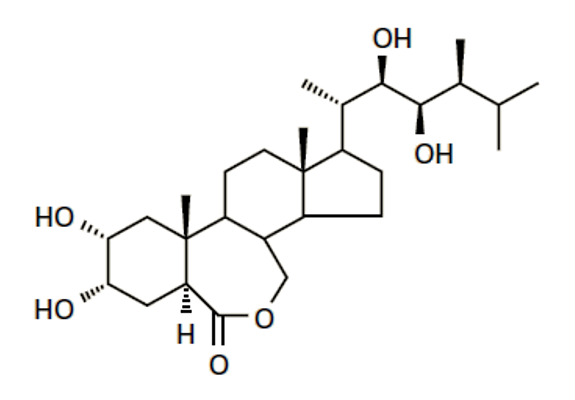
\includegraphics[width=.9\linewidth]{Imagenes/BL}
		\caption{}
		\label{BL}
	\end{subfigure}
	\begin{subfigure}{.4\textwidth}
		\centering
		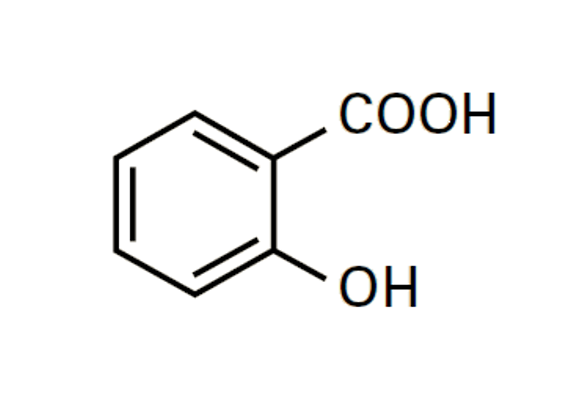
\includegraphics[width=.8\linewidth]{Imagenes/AS}
		\caption{}
		\label{AS}
	\end{subfigure}
	\caption{Estructura de hormonas vegetales, modificado de \cite{buchanan2015biochemistry} \\ a) Brasin\'olida (BL) y b) \'Acido salic\'ilico (AS).}
	\label{hormonas}
\end{figure}

La BL está considerada como el brasinoesteroide natural más activo descubierto hasta la fecha \citep{grove1979brassinolide}. Desafortunadamente, su concentración en fuentes naturales es baja, y tanto su purificación de fuentes vegetales como su síntesis orgánica constituye un proceso bastante costoso \citep{moreno2018silico}. Por tanto, se han buscado otras alternativas basadas en la síntesis de nuevas moléculas con alto grado de actividad biológica con bajos costos de producción \citep{lei2017structure}.\\

En este sentido, el laboratorio de Bioproductos del Centro de Investigación de Productos Naturales (CNPR) de la Facultad de Química de la Universidad de la Habana, ha desarrollado diversos productos a partir de saponinas y fitoesteroles de plantas, y mediante ensayos de actividad biológica se ha observado que algunos de estos tienen efectos naturales similares a BRs \citep{moreno2018silico}. Se analizaron, mediante métodos computacionales, la afinidad y las formas de unión de estos compuestos sintéticos análogos de BRs a su receptor BRI1 e indicaron que 17 de ellos pueden ser considerados buenos candidatos para la realización de pruebas biológicas. Entre estos análogos funcionales se destacan dos compuestos, DI-31 y MH-5 (Fig. \ref{br}), que han arrojado resultados prometedores en el efecto de estos compuestos en la defensa de las plantas frente al ataque por patógenos.\\

\begin{figure}[h!!!!]
	\begin{subfigure}{.5\textwidth}
		\centering
		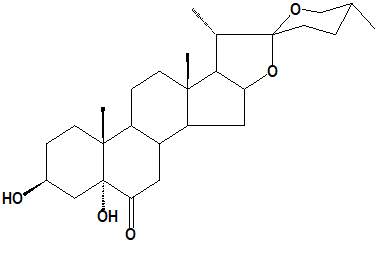
\includegraphics[width=.8\linewidth]{Imagenes/DI-31}
		\caption{}
		\label{di}
	\end{subfigure}
	\begin{subfigure}{.5\textwidth}
		\centering
		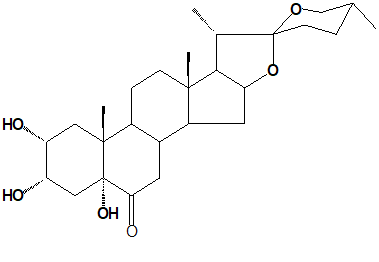
\includegraphics[width=.8\linewidth]{Imagenes/MH-5}
		\caption{}
		\label{mh}
	\end{subfigure}
	\caption{Estructura de an\'alogos sint\'eticos de BRs a) DI-31 y b) MH-5.}
	\label{br}
\end{figure}

\subsubsection{\'Acido salic\'ilico (AS).} 

El AS (Fig. \ref{AS}) es una hormona vegetal de naturaleza fen\'olica que participa en varias respuestas fisiol\'ogicas \citep{raskin1992salicylate} y se asocia con la activaci\'on de prote\'inas que participan en las respuestas de defensa \citep{glazebrook2005contrasting}.\\

En la literatura existen abundantes informes de la funci\'on del AS en la defensa contra distintos tipos de estr\'es abi\'otico, como los producidos por metales pesados \citep{alyemeni2014effect}, bajas temperaturas \citep{mutlu2013protective}, sequ\'ias \citep{alam2013exogenous} y salinidad \citep{fayez2014improving}, mediante el aumento de la actividad de las enzimas de defensa antioxidante. \\

\section{Especies reactivas del ox\'igeno (ROS).}

Las especies reactivas del ox\'igeno (ROS) son metabolitos del ox\'igeno molecular \citep{pandey2014oxidative}  que se generan en las plantas como consecuencia inevitable de las reacciones metab\'olicas aerobias \citep{buchanan2015biochemistry} o como respuesta de defensa. El ox\'igeno molecular es generalmente inactivo debido a la configuraci\'on de sus electrones \citep{elstner1987metabolism}, pero a diferencia de este, las ROS son mol\'eculas inestables y altamente reactivas. Entre las ROS se incluyen radicales del ox\'igeno: ani\'on super\'oxido $(O_{2}^{-} \bullet)$, radical hidroxilo $(OH\bullet)$ y radical perhidroxilo $(O_2H\bullet)$ y otras moléculas como el peróxido de hidrógeno $(H_2O_2)$ y el singlete de oxígeno $(^1O_2)$ \citep{buchanan2015biochemistry}.

\subsection{Producci\'on de ROS.}

En las plantas, la formaci\'on de ROS se lleva a cabo en diferentes compartimentos celulares \citep{apel2004reactive} e implica la fuga de electrones desde las cadenas transportadoras hacia el diox\'igeno \citep{corpas2015production}. Los cloroplastos y los peroxisomas son los principales productores en presencia de luz, mientras que la mitocondria es su principal fuente en condiciones de oscuridad \citep{choudhury2013reactive}. \\

El ani\'on super\'oxido se produce principalmente en  mitocondrias, apoplastos y en el fotosistema I (PSI) de los cloroplastos, mientras que el per\'oxido de hidr\'ogeno se genera en los peroxisomas \citep{gechev2006reactive, halliwell2006reactive}. \\

El singlete de ox\'igeno se produce principalmente en el fotosistema II de los cloroplastos. Su formación estimula la producción de  otras ROS \citep{buchanan2015biochemistry}, pero no se relaciona con la transferencia de electrones, ya que es el primer estado excitado del diox\'igeno, producido mediante fotoactivaci\'on \citep{triantaphylides2009singlet}. \\
 
%The chloroplast consists of a highly ordered system of thylakoids, which harbors the efficient light-capturing photosynthetic machinery. Photosystem (PS) I and PSII form the core of the light-harvesting systems in the thylakoids and are the primary sources of ROS generation [60, 61]. Near the reaction centers of PSII, O2 may produce 1O2 when there is overexcitation of chlorophyll under stress conditions. Besides, O2 •- may also be formed at PSI via Mehler reaction [62] or at PSII during electron transfer to O2 through QA and QB [55]. Additionally, due to the activities of flavin oxidases, peroxisomes are themain sites ofH2O2 generation [58, 63]. In mitochondria, O2 •- andH2O2 may be generated by univalent reduction of O2 near electron transport chain in plant cell [57]. 
%Apart from those organelles, there are cellular sites mediated in the generation of ROS. At plasmamembrane that plays a vital role in sensing environmental conditions, localized NADPH-dependent oxidase transfers electrons from NADPH on cytoplasmic side to O2 producing O2 •- [59]. ER also mediates the generation ofO2 •- by Cyt P450 [64].During harsh environmental conditions, the apoplast is rendered for H2O2 production by stress signals combined with ABA [65]. As cell wall localized peroxidase(s), diamine/polyamine oxidases and oxalate oxidase produceH2O2 that may, in turn, bemetabolized to OH• by the activity of class III peroxidases [66, 67]. 

Como se muestra en la figura \ref{ProdROS}, la reducción del $O_2$ ocurre a trav\'es de una secuencia de pasos. La primera reducción produce radicales superóxido o hidroperóxido. Posteriormente, el super\'oxido es dismutado a per\'oxido de hidr\'ogeno, lo cual puede ocurrir de forma espont\'anea (por p\'erdida de un electr\'on) o mediante la acci\'on de la enzima Super\'oxido Dismutasa (SOD) \citep{gechev2006reactive}. El per\'oxido de hidr\'ogeno producido puede ser transformado al radical hidroxilo en presencia de metales de transición como el hierro (Fe), mediante las reacciones de Haber-Weiss (o de Fenton) \citep{dat2000active}. Este tambi\'en puede ser eliminado por acción de la enzima catalasa (CAT) o del ciclo ascorbato-glutatión \citep{blokhina2003antioxidants, rinalducci2008redox}.\\

\begin{figure}[hbtp]
	\centering
	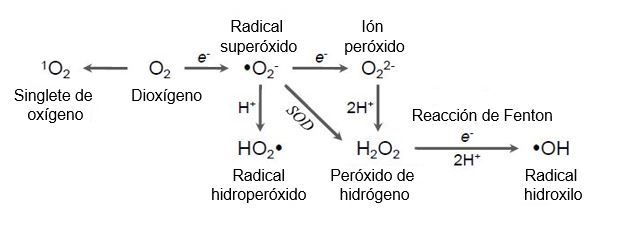
\includegraphics[scale=0.75]{Imagenes/ROSprod}
	\caption{Producci\'on de ROS durante la reducci\'on del ox\'igeno molecular. Modificado de \cite{imlay2008cellular, gill2010reactive}. }
	\label{ProdROS}
\end{figure}

\subsection{Efectos de ROS.}

Cuando los niveles de ROS son bajos o moderados funcionan como segundos mensajeros que median una serie de reacciones en las c\'elulas de las plantas, incluyendo el cierre de los estomas, la muerte celular programada (PCD, por sus siglas en ingl\'es) \citep{petrov2015ros}, gravitropismo \citep{wassim2013putative} y la adquisici\'on de tolerancia a estr\'es bi\'otico y abi\'otico \citep{nath2017reactive}. Pero el incremento de los niveles de ROS afecta una amplia variedad de funciones celulares, fisiol\'ogicas y bioqu\'imicas como la alteraci\'on de la membrana plasm\'atica, peroxidaci\'on lip\'idica, desnaturalizaci\'on de prote\'inas y destrucci\'on de ADN, ARN, enzimas y pigmentos \citep{xie2019roles}.\\
 
Aunque todas las ROS son muy reactivas, al poseer diferentes propiedades cada una puede reaccionar con diferentes biomol\'eculas \citep{peralta2012defensa}.\\

El ani\'on super\'oxido puede inactivar enzimas con centros hierro-azufre (Fe-S), mientras que el per\'oxido de hidr\'ogeno, aunque es relativamente estable, puede provocar la oxidación de grupos tiólicos e inactivar enzimas de esta manera. El radical perhidroxilo puede atravesar membranas y oxidar lípidos por la sustracción de protones de ácidos grasos poli-insaturados (PUFA). Por otra parte, el singlete de ox\'igeno es particularmente reactivo con dobles enlaces conjugados como los presentes en PUFA y aminoácidos aromáticos \citep{mittler2002oxidative, moller2007oxidative}.\\

Las propiedades tóxicas del super\'oxido y el per\'oxido de hidr\'ogeno aumentan en presencia de metales de transici\'on, ya que forman el radical hidroxilo que es la ROS más reactiva. Este radical tiene la capacidad de reaccionar rápidamente con todo tipo de macromoléculas y al no existir un mecanismo enzimático que la elimine, su sobreproducción finalmente conduce a la muerte de la c\'elula \citep{moller2007oxidative, sharma2009relationship, gill2010reactive}.\\

En cualquier caso, si la concentración intracelular de las ROS no es controlada, la consecuencia directa es el daño a estructuras celulares debido a la peroxidación de lípidos, oxidación de proteínas y componentes del ADN, así como la interrupción de rutas metabólicas \citep{moller2007oxidative, imlay2008cellular}.\\

\section{Estr\'es oxidativo.}

Existen v\'ias de eliminaci\'on que metabolizan las ROS y de esta forma controlan su concentraci\'on. Sin embargo, un desbalance en la generaci\'on y metabolismo de los niveles de ROS, interrumpe la homeostasis celular conduciendo a una variedad de retos fisiol\'ogicos que de forma general se conocen como \textquotedblleft estr\'es oxidativo\textquotedblright \citep{pandey2014oxidative}.\\

En las c\'elulas vegetales, el mayor da\~no oxidativo se produce en prote\'inas y l\'ipidos.  La actividad de las prote\'inas se altera mediante modificaciones en su estructura \citep{grimm2012oxidative}, mientras que los l\'ipidos, generalmente los poliinsaturados, pueden experimentar un proceso de descomposici\'on oxidativa en la membrana plasm\'atica, conocido como peroxidaci\'on lip\'idica \citep{catala2016impact, gaschler2017lipid}. Se ha demostrado que la peroxidaci\'on lip\'idica desencadena una serie de reacciones que producen otras mol\'eculas altamente reactivas, como cetonas, aldeh\'idos y mon\'oxido de hidr\'ogeno; adem\'as, puede modificar prote\'inas mediante la oxidaci\'on de algunos residuos aminoac\'idicos \citep{farmer2013ros, reginato2015role}.

\subsection{Mecanismos de resistencia}

Debido a los efectos da\~ninos que puede producir un desbalance de ROS, las plantas poseen un sistema de defensa antioxidante eficiente que evita el da\~no oxidativo y a la vez garantiza las funciones de se\~nalizaci\'on de las ROS \citep{liu2009oxidative, gill2010reactive}. Este sistema de defensa est\'a compuesto por mecanismos enzimáticos y no enzimáticos altamente regulados, que mantienen un balance entre la producción y eliminación de ROS, con el objetivo de mantener la homeostasis redox de la célula \citep{moller2001plant}.

\subsubsection{Mecanismos no enzim\'aticos}

Los antioxidantes no enzimáticos en plantas incluyen: ascorbato, glutati\'on reducido, taninos, flavonoides, $\alpha -$tocoferol, carotenoides y precursores de la lignina \citep{apel2004reactive}, que act\'uan a trav\'es de una serie de reacciones redox y evitan el da\~no oxidativo \citep{blokhina2003antioxidants}.\\

Los carotenoides y flavonoides neutralizan algunas ROS, entre las que se incluyen el per\'oxido de hidr\'ogeno y el singlete de ox\'igeno. El ascorbato es el antioxidante hidrosoluble m\'as abundante y poderoso que protege las membranas. El glutatión reducido constituye un importante mecanismo antioxidante y est\'a involucrado en algunas funciones vitales dentro de la c\'elula \citep{mittler2002oxidative}. El $\alpha-$tocoferol es el principal antioxidante liposoluble en las membranas fotosint\'eticas donde protege contra la peroxidaci\'on lip\'idica \citep{gechev2006reactive}. 

\subsubsection{Mecanismos enzim\'aticos}

Los mecanismos enzimáticos incluyen a las enzimas superóxido dismutasa (SOD), catalasa (CAT), ascorbato peroxidasa (APX), monodihidroascorbato reductasa (MDHAR), guaiacol peroxidasa (POX), glutatión reductasa (GR) y glutati\'on peroxidasa (GPX) \citep{ruley2004antioxidant}. \\

La SOD constituye la primera línea de defensa contra las ROS y es la \'unica enzima en plantas que dismuta el ani\'on super\'oxido en per\'oxido de hidr\'ogeno. El per\'oxido de hidr\'ogeno puede ser directamente catabolizado por CAT, o en presencia de sustratos reductores por varios tipos de peroxidasas, en el ciclo ascorbato$-$glutati\'on \citep{halliwell2006reactive}.\\

La extensión del estrés oxidativo en una célula está determinada por la cantidad de superóxido, per\'oxido de hidr\'ogeno y radicales hidroxilo. Por lo tanto, el balance de las actividades de SOD y CAT es crucial para suprimir los niveles tóxicos de ROS en la célula \citep{benezer2008produccion}. \\

\section{Enzimas de defensa en plantas.}

\subsection{Super\'oxido Dismutasa (SOD) (EC 1.15.1.1).}

Las Superóxido Dismutasas son una familia de metaloenzimas, descritas por primera vez por \cite{mccord1969superoxide}, que constituyen la primera línea de defensa antioxidante contra las ROS, catalizando la reacci\'on:
$$2O_2^- \; + \; 2H^+ \; \longrightarrow \; H_2O_2 \; + \; O_2$$

Existen tres isoformas de la enzima que son clasificadas de acuerdo al i\'on met\'alico presente en el centro activo: cobre/zinc (SOD Cu/Zn), hierro (SOD Fe) y manganeso (SOD Mn). Estas isoenzimas est\'an distribuidas en diferentes compartimentos celulares, probablemente porque el ani\'on super\'oxido no puede difundir a trav\'es de las membranas \citep{takahashi1983superoxide}, por lo que debe ser eliminado en su sitio de producci\'on. La comparaci\'on de las secuencias y estructuras de estas isoformas indican que SOD Mn y SOD Fe están estrechamente relacionadas, mientras SOD Cu/Zn parecen haber evolucionado independientemente \citep{bowler1994superoxide}.\\

La isoforma SOD Cu/Zn es la más abundante en organismos eucariotas y está localizada principalmente en el citoplasma, en los cloroplastos y en diferentes tipos de peroxisomas. También se encuentran en el núcleo y en el apoplasto. La isoforma SOD Mn se ha encontrado en mitocondrias y peroxisomas, mientras que la isoforma SOD Fe está presente en los cloroplastos \citep{munoz2005crystal}.\\

Para cada isoforma el mecanismo de cat\'alisis es similar e involucra un bolsillo o pliegue rodeado de residuos aminoac\'idicos cargados positivamente que atraen al ani\'on super\'oxido hacia el centro activo de la enzima. El metal de transici\'on presente en el centro activo lleva a cabo una transferencia de electrones entre dos aniones super\'oxido \citep{bowler1994superoxide}. \\

\subsection{Catalasa (CAT) (EC 1.11.1.6).}

La catalasa ($H_2O_2$:$H_2O_2$ oxidorreductasa) es una hemoprote\'ina tetram\'erica que est\'a presente en la mayor\'ia de los organismos aerobios. Adem\'as, es una de las enzimas principales en el catabolismo del per\'oxido de hidr\'ogeno \citep{luhova2003activities}. \\

Las CAT de plantas se encuentran mayormente en los peroxisomas \citep{luhova2003activities} y existen varias isoformas de la enzima, lo que sugiere que posee m\'ultiples funciones \citep{scandalios1997catalases}.\\

En dependencia de la concentraci\'on de per\'oxido de hidr\'ogeno, la CAT puede ejercer una funci\'on dual \citep{deisseroth1970catalase}. A bajas concentraciones puede actuar peroxidativamente, donde varias sustancias como el etanol y el \'acido asc\'orbico pueden ser oxidadas siguiendo la reacci\'on:

$$RH_2 \; +\; H_2O_2 \; \rightarrow \; R \; + \; 2H_2O $$

Mientras que a altas concentraciones de sustrato la CAT descompone r\'apidamente el per\'oxido de hidr\'ogeno mediante la reacci\'on catal\'itica:

$$2H_2O_2 \; \rightarrow \; 2H_2O \; + \; O_2$$

Evidencias cin\'eticas y espectrofotom\'etricas sugieren que la CAT utiliza un mecanismo de dos pasos en estas reacciones \citep{deisseroth1970catalase, dounce1983proposed}. \\

En la reacci\'on catal\'itica, la CAT presenta una constante de Michaelis-Menten muy elevada, en consecuencia, la enzima no se satura f\'acilmente con sustrato. De esta manera, la actividad enzim\'atica aumenta linealmente frente a una amplia gama de concentraciones de per\'oxido de hidr\'ogeno, lo que le permite controlar la concentraci\'on intracelular de esta ROS \citep{scandalios1997catalases}.\\




\subsection{Polifenol oxidasa (PPO) (EC 1.10.3.1).}

Las PPO son una familia de metaloenzimas monom\'ericas que reaccionan con una amplia gama de sustratos fen\'olicos. El centro activo de la enzima consiste en dos \'atomos de cobre, cada uno acoplado con tres residuos de histidina conservados \citep{lerch1983neurospora, huber1985primary}.\\

Las PPO se encuentran en la membrana de los tilacoides de los cloroplastos  y son liberadas al citoplasma ante daños mecánicos en la estructura tisular y celular que pueden ocurrir durante la senescencia, lesiones o estr\'es \citep{marshall2000enzymatic, mayer2006polyphenol}. Esto conduce al contacto de la enzima con compuestos fen\'olicos que son liberados desde la vacuola, donde se encuentran almacenados \citep{queiroz2008polyphenol}. La actividad catal\'itica de la enzima est\'a influenciada por caracter\'isticas estructurales de los sustratos, como la naturaleza de la cadena lateral y el n\'umero de grupos hidroxilo y la posici\'on que ocupan en el anillo de benzeno \citep{macheix1990phenolic}.\\

La PPO cataliza dos reacciones (Fig. \ref{PO}): la o-hidroxilaci\'on de monofenoles a o-difenoles (actividad creolasa) y la oxidaci\'on de estos a o-quinonas (actividad catecolasa), utilizando el oxígeno molecular como agente oxidante \citep{jukanti2017distribution}.\\

\begin{figure}[hbtp]
	\centering
	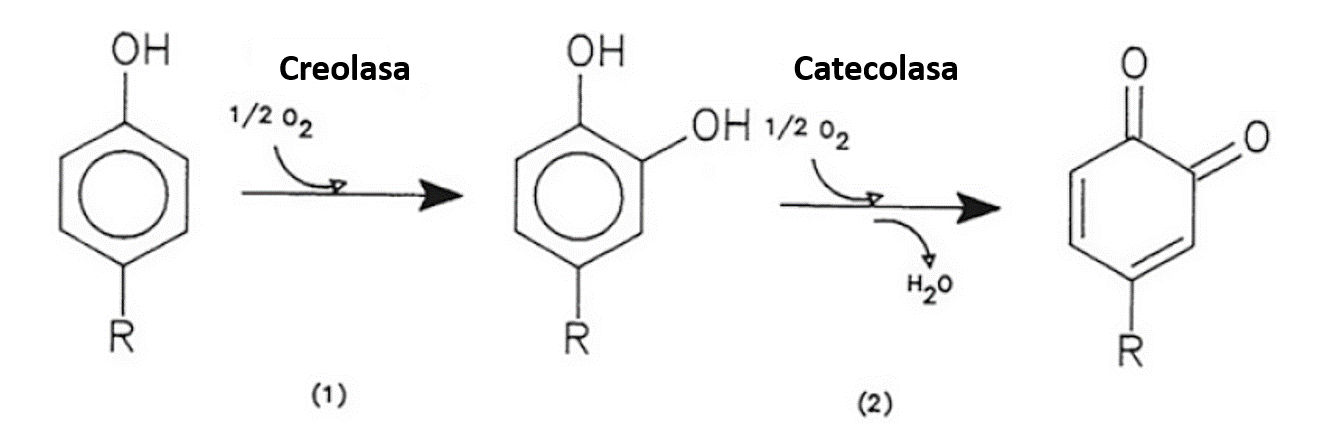
\includegraphics[scale=0.65]{Imagenes/PO}
	\caption{Actividad creolasa (1) y catecolasa (2) de PPO. Modificado de \cite{nicolas1994enzymatic}. }
	\label{PO}
\end{figure}

Las o-quinonas generadas son altamente reactivas e inestables \citep{mayer2006polyphenol} y pueden reaccionar con grupos amino y tiol de aminoácidos libres y proteínas mediante mecanismos no enzimáticos, o reaccionar covalentemente con otros compuestos fenólicos para formar diferentes pigmentos, ocasionando así el efecto conocido como pardeamiento enzimático \citep{kumar2008purification}. Este efecto es muy com\'un en frutas y verduras y ha sido propuesto como mecanismo de defensa contra pat\'ogenos e insectos \citep{mayer1979polyphenol, vaughn1988polyphenol}.\\

Las PPO han sido implicadas en las respuestas de defensa de las plantas debido a la aparici\'on de sus productos de reacci\'on en el momento de ataques de pat\'ogenos e insectos, lesiones y diferentes tipos de estr\'es \citep{mayer1979polyphenol, constabel1995systemin, maki2006development}. Adem\'as, se ha identificado que aplicaciones ex\'ogenas de BRs aumentan la tolerancia de plantas a diferentes tipos de estr\'es, mediante el incremento de la actividad de PPO \citep{sharma2010regulation, sharma2012effect, el2012brassinolide}.\\

\section{Par\'ametros experimentales.}

En la figura \ref{curva} se muestra la velocidad máxima inicial ($V_{max}$) a una concentración determinada de enzima $[E_o]$. Este par\'ametro cin\'etico posee las mismas unidades de v$_o$ y representa la máxima eficiencia catalítica de una enzima frente a un sustrato específico, a la concentración de enzima y valores de pH, fuerza iónica y temperatura utilizados experimentalmente \citep{chavez1990temas}.\\

\begin{figure}[hbtp]
	\centering
	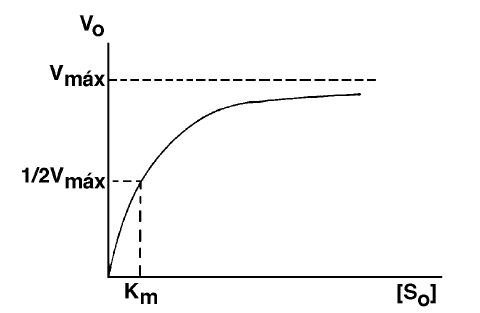
\includegraphics[scale=0.8]{Imagenes/curva}
	\caption{Representación gráfica de v$_o$ en función de $[S_o]$, a $[E_o]$ constante, para una reacción enzimática monosustrato, a partir de la ecuación de Michaelis-Menten. $V_{max}$: velocidad máxima; $K_m$: constante de Michaelis \citep{chavez1990temas}.}
	\label{curva}
\end{figure}

En la figura \ref{curva} también se muestra el valor de $K_m$. Este par\'ametro cin\'etico representa la concentración inicial de sustrato $[S_o]$, que da lugar a una velocidad inicial igual a la mitad de la velocidad máxima y tiene las mismas unidades de $[S_o]$. El valor de $K_m$ es característico de una enzima frente a un sustrato particular y en las condiciones de pH, fuerza iónica y temperatura del experimento, pero no depende de la concentración de enzima \citep{chavez1990temas}.\\

El valor de $K_m$ medido de esta forma puede diferir de su valor verdadero, el cual es definido en términos de constantes de velocidad. Si hay presente inhibidores u otros factores, el valor medido debe ser denominado $K_m \; aparente$ \citep{chavez1990temas}. \\

En las condiciones de cumplimiento del equilibrio de Michaelis-Menten, cuando $K_m$ = $K_s$ el valor de $K_m$ puede reflejar la mayor o menor afinidad de una enzima por un sustrato. Esta relación es inversa, por tanto, a mayor valor de $K_m$ más concentración de sustrato se requiere para alcanzar la mitad de $V_{max}$ y viceversa \citep{chavez1990temas}.\\

%%KM es una constante de disociación aparente que puede ser tratada como una constante global de disociación de todos los complejos enzimáticos intermediarios\citep{chavez1990temas}.

%ks constante de saturaci\'on

En este trabajo, no es posible determinar la $K_{cat}$ debido a que la enzima no est\'a purificada, por lo que se trabajar\'a con $V_{max}$ . Por este motivo, tampoco se puede determinar el valor real de $K_m$, por lo que el valor obtenido para este par\'ametro ser\'a referido como $K_ma$ y ser\'a utilizado para caracterizar las enzimas. \\

%Evaluaremos la afinidad de las enzimas por el sustrato
%
%1- La constante de Michaelis-Menten es un elemento de juicio importante para caracterizar una enzima.
%2- El Km indica la afinidad de la enzima por el sustrato. 


\section{\textit{Raphanus sativus} como modelo experimental.}

La selecci\'on de este modelo experimental se basa en el gran n\'umero de fuentes existentes en la literatura, donde son utilizadas plantas de r\'abano para estudiar el efecto de BRs en las enzimas de defensa vegetal. El r\'abano es considerado un cultivo modelo para el estudio de los efectos de distintos tipos de estr\'es, entre ellos h\'idrico  \citep{mahesh2013effect}, oxidativo \citep{sharma2012effect} y por metales pesados \citep{dhriti201424}. \\

Las plantas de r\'abano poseen un tiempo relativamente corto de germinaci\'on, as\'i como un bajo costo, lo que constituyen ventajas en su utilizaci\'on como modelo experimental. Adem\'as, numerosos estudios han corroborado el aumento de las enzimas de defensa de \textit{Raphanus sativus} al aplicar an\'alogos sint\'eticos de BRs. 


\chapter{Materiales y Métodos }

\section{Material vegetal.}

Como modelo experimental se utilizaron plantas de \textit{Raphanus sativus} (r\'abano). Las plantas se mantuvieron expuestas a la luz solar de forma indirecta, por un tiempo de aproximadamente $15$ días, manteniéndose  en condiciones constantes de luminosidad y de disponibilidad de agua y nutrientes. 

\section{Diseños experimentales.}

Se describen dos dise\~nos experimentales que permiten la evaluaci\'on de la actividad de las enzimas de defensa en plantas de \textit{R. sativus} sometidas y no sometidas a estr\'es salino. 

\subsection{Primer dise\~no experimental: Actividad enzim\'atica en plantas no sometidas a estr\'es salino.} \label{d1}

Para este experimento se utilizó un total de 15 plantas de r\'abano, divididas en 5 grupos experimentales (3 plantas por grupo): Control negativo (planta sin tratar), Etanol (EtOH) (0,01 mg/mL), DI-31 (0,01 mg/mL), MH-5 (0,01 mg/mL) y Ácido Salicílico (AS) (0,01 mg/mL) como control positivo del experimento (Fig. \ref{plantas}). \\

Para su cultivo se prepar\'o una mezcla de tierra/humus en partes iguales en un semillero germinador y se sembraron dos semillas en cada división. Cada grupo experimental fue sometido a un único tratamiento, los cuales fueron aplicados por aspersión foliar (con el uso de un nebulizador) en tres dosis: a las 0, 24 y 48 horas luego de comenzado el experimento.\\

Las hojas de las plantas se recolectaron a las 24, 48 y 72 horas después de haber comenzado el ensayo. Las muestras fueron maceradas en nitrógeno líquido y almacenadas a $-20^oC$ hasta su procesamiento. \\

%\begin{table}[h]
%	\caption{Esquema de trabajo para cada uno de los tiempos. El primer n\'umero asignado a cada planta representa el tiempo de recogida de la muestra y el segundo representa el tratamiento.}
%	\label{esquema1}
%	\begin{center}
%		\begin{tabular}{|c|M{25mm}|M{25mm}|M{25mm}|M{25mm}|M{25mm}|c|}
%			\hline 
%			\textbf{} & \textbf{Nada} & \textbf{EtOH} & \textbf{DI-31} & \textbf{MH-5} & \textbf{AS} \\ 
%			\hline 
%			$24 \; horas$ &  $Planta \; 1.1$ & $Planta\; 1.2$  & $Planta\; 1.3$ & $Planta\; 1.4$ & $Planta\; 1.5$ \\ 
%			\hline 
%			$48 \; horas$ &  $Planta\; 2.1$ & $Planta \;2.2$  & $Planta \;2.3$ & $Planta \;2.4$ & $Planta\; 2.5$ \\ 
%			\hline 
%			$72 \; horas$ &  $Planta \;3.1$ & $Planta \;3.2$  & $Planta \;3.3$ & $Planta \;3.4$ & $Planta \;3.5$ \\
%			\hline 
%		\end{tabular} 
%	\end{center}
%\end{table}
%
%\normalsize


\begin{figure}[hbtp]
	\centering
	\includegraphics[scale=0.70]{Imagenes/plantas}
	\caption{Primer dise\~no experimental: Plantas de \textit{Raphanus sativus} no sometidas a estr\'es salino. Tratamientos: AS, DI-31, EtOH y control negativo.}
	\label{plantas}
\end{figure}

\subsection{Segundo dise\~no experimental: Actividad enzim\'atica en plantas sometidas a estr\'es salino (NaCl).} \label{d2{}}

Este dise\~no se basa en la metodolog\'ia propuesta por \cite{muthukumarasamy2000enhancement} (con modificaciones) y permite estudiar el efecto de los compuestos DI-31 y MH-5 en la actividad de las diferentes enzimas ante estr\'es por salinidad. El dise\~no de los tratamientos se muestra en la tabla \ref{Ttos}. \\

\begin{table}[h]
	\caption{Dise\~{n}o de los tratamientos.}
	\label{Ttos}
	\begin{center}
		\begin{tabular}{|c|l|}
			\hline 
			\textbf{ } & \textbf{Tratamientos} \\ 
			\hline 
			1 & semillas con $H_2O$ destilada \\ 
			\hline 
			2 & NaCl  \\ 
			\hline 
			3 & NaCl + DI-31 ($1 \; mg/mL$) \\ 
			\hline 
			4 & NaCl + MH-5 ($1 \; mg/mL$) \\ 
			\hline 
			5 & NaCl + AS ($1 \; mg/mL$) \\ 
			\hline 
		\end{tabular} 
	\end{center}
\end{table}

\begin{figure}[hbtp]
	\centering
	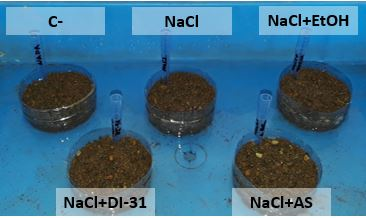
\includegraphics[scale=0.8]{Imagenes/plantas2}
	\caption{Segundo dise\~no experimental: Semillas de \textit{Raphanus sativus} previas a su germinaci\'on sometidas a estr\'es salino. Tratamientos: control negativo, NaCl, NaCl+EtOH, NaCl+DI-31 y NaCl+AS.}
	\label{plantas2}
\end{figure}

Para crear las condiciones de estr\'es salino se utiliz\'o una soluci\'on de NaCl $80\;mM$, ya que esta concentraci\'on disminuye la masa seca en un $50\%$ respecto al control \citep{muthukumarasamy2000enhancement}.\\

Previo a la siembra, se incubaron las semillas de r\'abano por tres horas en una soluci\'on que conten\'ia cada uno de los tratamientos utilizados, lo que constituye una de las diferencias fundamentales entre los dise\~nos experimentales propuestos. Est\'a ampliamente informado en la literatura que las incubaciones previas en agua o soluciones de varias sustancias afectan positivamente los rasgos tanto de la semilla, como del reto\~no \citep{burgass1984evidence, bradford1986manipulation, taylor1998seed, mcdonald2000seed}.\\

Posteriormente se sembraron diez semillas en cada recipiente relleno de una mezcla de tierra/humus en partes iguales. Los grupos experimentales fueron irrigados con las soluciones descritas anteriormente cada 5 días, durante un período de 30 días. Se recolectaron las hojas de las plantas a los 15 y 30 días después de la primera irrigación y se almacenaron a $-20^oC$ hasta su posterior procesamiento.

%\begin{table}[h]
%	\caption{Cronograma del experimento.}
%	\label{cron}
%	\begin{center}
%		\begin{tabular}{|c|l|}
%			\hline 
%			D\'ia 1 & Sembrado. Primera aplicaci\'on de los tratamientos. \\ 
%			\hline 
%			D\'ia 5 & Segunda aplicaci\'on de los tratamientos.  \\ 
%			\hline 
%			D\'ia 10 & Tercera aplicaci\'on de los tratamientos. \\ 
%			\hline 
%			D\'ia 15 & Recogida del primer grupo experimental.  Cuarta aplicaci\'on de los tratamientos  \\ 
%			\hline 
%			D\'ia 20 & Quinta aplicaci\'on de los tratamientos. \\ 
%			\hline 
%			D\'ia 25 & Sexta aplicaci\'on de los tratamientos. \\ 
%			\hline 
%			D\'ia 30 & Recogida del segundo grupo experimental. \\ 
%			\hline 
%		\end{tabular} 
%	\end{center}
%\end{table}
%
%\normalsize

\section{Metodolog\'ias para la extracci\'on de enzimas.}

Para la preparación de los extractos enzimáticos crudos se utilizaron dos protocolos diferentes. 

\subsection{Protocolo de extracci\'on propuesto por \cite{liu2010exogenous}, con modificaciones.} \label{p1}

Se maceraron $500 \; mg$ de tejido vegetal, utilizando un mortero de cerámica, en nitrógeno líquido, para mantener baja la temperatura y asegurar la ruptura tisular. A la muestra pulverizada se le añadió $1\;mL$ de la Solución de Extracción (Fosfato de Sodio $50\;mM$, EDTA dis\'odico $1\;mM$, $2\%$ Polivinil Pirrolidona (PVPP), pH 7.0; $4^oC$).\\

Las muestras fueron centrifugadas a $10\;000\;g$ por $5$ minutos. El sobrenadante fue transferido a tubos limpios y utilizado para la cuantificación de proteínas y los ensayos enzimáticos de SOD, CAT y PPO. \\

\subsection{Protocolo de extracci\'on propuesto por \cite{baquero2005catalase}, con modificaciones.} \label{p2}

En un mortero de cer\'amica se maceraron $500\;mg$ de material vegetal en nitr\'ogeno l\'iquido, para asegurar la baja temperatura y la ruptura tisular. \\

Una vez triturado el tejido, se a\~nadi\'o al mortero $1\;mL$ de Acetona pura para an\'alisis y se macer\'o nuevamente. El macerado se transfiri\'o a un tubo de microcentr\'ifuga, se incub\'o a $4^oC$ durante 30 minutos para obtener un precipitado proteico y se desech\'o el sobrenadante de acetona utilizando una micropipeta. Este proceso se realiz\'o nuevamente y el sobrenadante se elimin\'o mediante evaporaci\'on al vac\'io con un \textquotedblleft SpeedVac \textquotedblright. \\

El precipitado final se resuspendi\'o con $1\;mL$ de una soluci\'on tamp\'on de Fosfato de Potasio ($200\;mM$, pH 6.8) y se mantuvo bajo agitación continua por $24$ horas a $4^oC$. Posteriormente, las muestras se centrifugaron a 10 000 g durante 20 minutos y se desech\'o el precipitado. El sobrenadante fue utilizado para la cuantificación de proteínas y los ensayos enzimáticos de SOD y PPO.\\

\section{Determinaci\'on de la concentración de proteínas mediante el m\'etodo Bradford.}

La concentraci\'on de prote\'inas se determin\'o siguiendo la metodolog\'ia propuesta por \cite{bradford1976rapid}, con modificaciones. Se emple\'o el Reactivo de Bradford, el cual contiene como colorante Azul Coomassie Brillante G-250 (CBBG, por sus siglas en inglés). La Alb\'umina de Suero Bobino (BSA, según sus siglas en inglés) se emple\'o como prote\'ina est\'andar.  

\subsection {Medición de la proteína estándar.}

Partiendo de una soluci\'on $1\;mg/mL$ de BSA se prepararon diluciones seriadas, de manera que cada muestra analizada contaba con: $100\;\mu g$; $50\;\mu g$; $25\;\mu g$; $12.5\;\mu g$; $6.25\;\mu g$ y $3.125\;\mu g$. De cada diluci\'on fueron a\~nadidos $100 \;\mu L$ en tubos de ensayo diferentes y se adicion\'o el Reactivo de Bradford necesario para un volumen final de $3 \; mL$. Las muestras se incubaron durante 20 minutos a temperatura ambiente. La DO de cada muestra se midi\'o a $595 \;nm$ en un espectrofotómetro de luz visible (UV-1800 UV/Visible, China) \citep{kruger2009bradford}.

\subsection {Cuantificación de proteínas en el extracto enzim\'atico.}

Este proceso se realiz\'o de forma similar a la descrita anteriormente, utilizando un volumen del extracto enzim\'atico de concentraci\'on proteica desconocida, contenido en el intervalo analizado en la prote\'ina est\'andar. 

\section{Ensayos enzimáticos.} 

Se describen los protocolos utilizados para la medici\'on de la actividad de las enzimas SOD, CAT y PPO.

\subsection{Super\'oxido Dismutasa (SOD).}

La cuantificaci\'on de la actividad enzim\'atica de SOD se realiz\'o mediante el m\'etodo colorim\'etrico propuesto por \cite{ma2009spectroscopic}, con modificaciones.\\ 

Este m\'etodo se basa en la estimaci\'on de la inhibici\'on que produce la actividad de la enzima SOD en la autoxidaci\'on del Pyrogallol (\'acido 1,2,3-trihidroxibenzoico). El $50\%$ de la inhibici\'on es equivalente a una unidad de SOD  \citep{pandey2014oxidative}. \\

En una cubeta de vidrio se a\~nadieron $2\;700\;\mu L$ de soluci\'on tamp\'on Tris-HCl $50\;mM$ EDTA dis\'odico $1\;mM$ (pH 8.2), $100\;{\mu}L$ de extracto enzim\'atico y $200\;{\mu}L$ de Pyrogallol a diferentes concentraciones (10 mM; 6,4 mM; 3,2 mM; 1,6 mM y 0,8 mM), para un volumen final de $3\;000{\mu}L$ (3 mL). \\

La soluci\'on de Pyrogallol se prepar\'o a $15\;mM$ en $1\;M$ de HCl, solución que es posible almacenar hasta 3 meses \citep{masayasu1979simplified}. En el momento del ensayo, se diluyó a las concentraciones mencionadas anteriormente. \\

El blanco del experimento se prepar\'o a\~nadiendo todos los componentes del ensayo, excepto el extracto (que fue sustituido por $H_2O$ destilada) a fin de determinar la velocidad basal de autoxidación del Pyrogallol en la soluci\'on. Este proceso de inhibici\'on de la autoxidaci\'on del Pyrogallol se monitore\'o a partir de la medici\'on de la DO a $240\;nm$, cada 15 segundos, durante 3 minutos, a $25^oC$, en un espectrofotómetro de luz visible (UV-1800 UV/Visible, China). \\

%Auto-oxidation of pyrogallol was monitored by recording the kinetics of the reaction mixture containing 2.94 ml of Tris-HCl buffer (50 mM, pH 8.2) 1 mM DETAPAC (Sigma) and 60 µl pyrogallol (20 mM prepared in 10 mM HCl ), on a UV-VIS spectrophotometer (ATI - Unicam, UK) at 420 nm. For SOD assay, 0.2 ml enzyme extract was added to 2.74 ml of the Tris-HCl buffer and the absorbance was adjusted to zero. The reaction was initiated by adding 60 µl of pyrogallol and the change in absorbance was recorded at 420 nm.

Para el c\'alculo de la actividad de SOD, se utilizaron los valores de DO obtenidos tanto para el blanco, como para la muestra. Para ello se siguieron las siguientes ecuaciones, en el orden referido \citep{pandey2014oxidative}:

\begin{equation}
Tasa \; de \; autoxidaci\acute{o}n \; del \; Pyrogallol =\frac {[DO(420) \; final \; - \; DO(420) \; inicial]} {[Tiempo \; de \; ensayo \; (min)]}
\label{tasapyr}
\end{equation}

\begin{equation}
Tasa \; de \; SOD =\frac {[DO(420) \; final \; - \; DO(420) \; inicial]} {[Tiempo \; de \; ensayo \; (min)]}
\label{tasasod}
\end{equation}

\begin{equation}
Inhibici\acute{o}n \; (I) ={Tasa \; de \; autoxidaci\acute{o}n \; del \; Pyrogallol} - {Tasa \; de \; SOD}
\label{inh}
\end{equation}

\begin{equation}
Inhibici\acute{o}n = {\frac{Inhibici\acute{o}n \; (I)} {Tasa \; de \; autoxidaci\acute{o}n \; del \; Pyrogallol} * 100}
\label{inhporc}
\end{equation}

\begin{equation}
50\% \; de \; Inhibici\acute{o}n ={1 \; unidad \; de \; SOD} \rightarrow \% \; Inhibici\acute{o}n \;  \; de \;  X  = \frac{X}{50} \; unidades \; de \; SOD
\label{50inh}
\end{equation}

\begin{equation}
Factor \; de \; diluci\acute{o}n \; 1 = \frac{V (de \; la \; mezcla \; de \; ensayo)}{V (del \; extracto \; enzim\acute{a}tico \; en \; la\; mezcla \; de \; ensayo)}
\label{fd1}
\end{equation}

\begin{equation}
Factor \; de \; diluci\acute{o}n \; 2 = \frac{V (total \; del \; extracto \; enzim\acute{a}tico)}{V (del \; extracto \; enzim\acute{a}tico \; utilizado \; en\; el \; ensayo)}
\label{fd2}
\end{equation}

\begin{equation}
Factor \; de \; diluci\acute{o}n \; total \; (FD) ={Factor \; de \; diluci\acute{o}n \; 1 \; * \; Factor \; de \; diluci\acute{o}n \; 2}
\label{FD}
\end{equation}

\begin{equation}
Actividad \; de \; SOD \; (unidades \; mg^{-1} \; MF) = \frac{unidades \; de \; SOD \; * \; FD}{MF \; de \; la \; muestra} 
\label{act}
\end{equation}

\medskip
\medskip

El Factor de Diluci\'on 2 (Ecuaci\'on \ref{fd2}) no se utiliz\'o en este ensayo, pero es importante para el c\'alculo de la actividad enzim\'atica total de una planta o de un \'organo completo de la misma.

\subsection{Catalasa (CAT).}

Para la cuantificación de la actividad CAT, se sigui\'o la metodolog\'ia propuesta por \citep{chance1955136}, con modificaciones. \\

El extracto enzim\'atico utilizado fue el obtenido mediante el protocolo de extracci\'on propuesto por \cite{liu2010exogenous}, con modificaciones. En una cubeta de cuarzo se a\~nadieron $1\;500\;{\mu}L$ de soluci\'on tamp\'on Fosfato de Potasio $50\;mM$ (pH 7.0), $500\;{\mu}L$ de $H_2O_2$ a dos concentraciones diferentes ($5\;mM$ y $50\;mM$) y $100\;{\mu}L$ de extracto enzimático, para un volumen final de $3\;000\;{\mu}L$ ($3\;mL$). Se utiliz\'o como blanco los mismos componentes referidos anteriormente, con excepción del extracto enzimático (que fue sustituido por $H_2O$ destilada). \\

El $H_2O_2$ $30\%$ se diluy\'o en soluci\'on de Fosfato de Potasio $50\;mM$, en el momento del ensayo. Se ajust\'o la DO de esta solución a $2,05\;cm^{-1}$. Se monitore\'o la disminución de  $H_2O_2$ a partir del decremento de absorbancia, utilizando un espectrofotómetro de luz ultravioleta (\textit{Thermo Scientific spectronic Genesys 10UV}, Estados Unidos) a $240\;nm$ a intervalos de 15 segundos, durante 5 minutos, a $25^oC$. \\

Para calcular la actividad enzimática espec\'ifica se utiliz\'o el coeficiente de extinción del  $H_2O_2$ $39.4\;mM^{-1}cm^{-1}$ y se expresa en $nmol$ de $H_2O_2$ por miligramo de masa fresca (MF) por minuto $(nmol (H_2O_2)mg^{-1}MF^{-1}min^{-1})$.

%ACTIVIDAD CATALASA

%Mezcla de reacción (en cubeta de cuarzo)
%.
%Blanco	Muestra
%Buffer fosfato 50 mM pH 7	1.6 mL	1.5 mL
%%H2O2  50 mM	500 L	500  L
%%Extracto enzimático	--	100  L
%
%%Añada 1,5 mL de solución amortiguadora a la cubeta, 500 µL de H2O2 50mM  y 100 μL de muestra, tape y homogenice por inversión. Lea a los 10 y 70 seg. a 240nm.
%%Siga el procedimiento anterior para determinar la diferencia de densidad óptica que se produce al  reemplazar los 100 L de muestra por solución amortiguadora de fosfato (blanco). Antes de leer el  blanco ajustar a cero absorbancia con solución amortiguadora de fosfato.
%Nota: En presenciasdeactividad Enzimática se observa unadisminuciónela densidad  ópticadelmedio
%NotA: SI CON ESTAS CANTIDADES NO DA BIEN PROBAR  CON LA METODOLOGIA Y CONCENTRACIONES DADAS POR BIOCHEMICA INFORMATION
%
%Cálculos
%Calcule inicialmente:
%%ΔDOmuestra= DO70seg_DO10seg
%%ΔDOblanco= DO70seg_DO10seg
%%Se utilizara el coeficiente de extinción 40 mM-1 cm-1 para el  H2O2 a una λ=240nm 
%%CmM = DO/ ε b
%%donde ε esel chef deextinción y b es el paso deluz de la cubeta: 1cm
%%[(ΔDOmuestra_ ΔDOblanco)] / (40 mM-1 cm-1. cm) = concentración (mmol) de H2O2 descompuesta en un tiempo de 60 segundos (1 minuto) por cada litro de solución.
%%Si tenemos en cuenta del volumen total de la cubeta en la misma se descompuso una cantidad de peroxido igual a:
%
%%[(ΔDOmuestra_ ΔDOblanco)] = A
%
%[A/40] . 2.1/1000 = milimoles de peroxido descompuesto en la cubeta. Esta descomposición fue provocada por 100 microlitors del extracto enzimático.
%Ahora hay que conocer que cantidad de proteína hay en ese volumen d3e extracto enzimatico para expresar la actividad en función de la proteína.
%
%Referencias
%1- Boehringer Mannheim. Biochemical Information. A revised biochemical reference source. Enzymes for routine (1st edition), Germany: Boehringer Mannheim, 1987:15-16.
%
%2- Biochemica Information II 167 pp (pág 47), Bergmeyer, H.U (1955) Biochem, Z. 327, 255
%
%3- Kato M. and S. Shimizu (1987) Chlorophyll metabolism in higher plants. VII chlorophyll degradation in senescing tobacco leaves phenolic-deppendent peroxidative degradation Can J Bot 65: 729-735 Ver Lin nd kao 1998 en file Metodologías antioxidantes.


\subsection{Polifenol Oxidasa (PPO).}

La actividad de la enzima polifenol oxidasa se determin\'o siguiendo la metodolog\'ia descrita por \cite{baquero2005catalase}, con modificaciones.\\

Este ensayo se realizó utilizando un Espectrofotómetro de placas \textit{FLUOstar OPTIMA (BMG LABTECH}, Alemania), lo que permitió reducir en gran medida el volumen final del ensayo ($200\;\mu L$). La mezcla de reacción consistió en $100\;\mu L$ de extracto enzimático más $100\;\mu L$ de L-DOPA disuelto en solución de Fosfato de Potasio 200 mM, pH 7.0. Las concentraciones de sustrato utilizadas fueron 10 mM; 7 mM; 5 mM; 2,5 mM y 1,25 mM. Se utilizó como blanco los mismos componentes referidos anteriormente, con excepción del extracto enzimático (que fue sustituido por $H_2O$ destilada). La reacción se monitoreó por 2 minutos, a intervalos de 10 segundos, a $25^oC$ y a una longitud de onda de 475 nm. \\

Una  unidad de actividad fue definida como el cambio en una unidad de absorbancia por minuto. La actividad específica fue expresada en unidades de actividad por miligramo de proteína.

\section{Procesamiento matem\'atico.}

Para la realizaci\'on de la curva t\'ipica y de los gr\'aficos de barra se utiliz\'o el programa \textit{Microsoft Excel 2013}. \\

Se realiz\'o un ANOVA simple mediante el programa \textit{PAST} \citep{hammer2001past}, para comparar las concentraciones de prote\'inas de los extractos utilizados para medir la enzima SOD. \\

Se emple\'o el programa \textit{GraphPad Prism 5} \citep{motulsky2007prism} para la confecci\'on de las curvas de cin\'etica enzim\'atica Michaelis-Menten.



\chapter{Resultados}

\section{Determinaci\'on de la cantidad de prote\'inas.}

La curva de calibraci\'on obtenida por el m\'etodo de \cite{bradford1976rapid} (Fig. \ref{bsa}) es la de una ecuaci\'on de regresi\'on lineal. El valor del coeficiente $R^2$ muy cercano a 1 refleja un buen ajuste lineal de los datos. Los valores de concentraci\'on de prote\'inas se especifican para cada uno de los extractos.

\begin{figure}[hbtp]
	\centering
	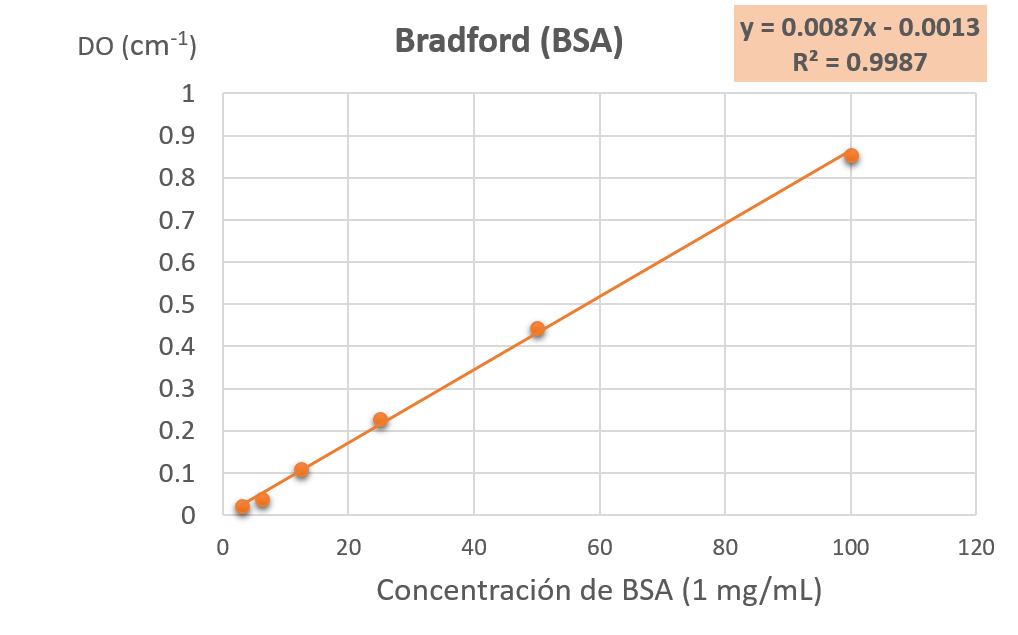
\includegraphics[scale=0.80]{Imagenes/BSA}
	\caption{Representaci\'on de DO obtenida por el reactivo Bradford y la concentraci\'on de Alb\'umina de Suero Bovino.}
	\label{bsa}
\end{figure}

\section{Enzima Super\'oxido Dismutasa (SOD).}

La actividad de la enzima SOD, para los diferentes tratamientos, se determin\'o en plantas no sometidas a estr\'es salino (primer dise\~no experimental). 

\subsection{Actividad enzim\'atica de SOD en extractos obtenidos mediante protocolo de extracci\'on enzim\'atica propuesto por \cite{liu2010exogenous}, con modificaciones.}

La concentraci\'on de prote\'inas de los extractos obtenidos para cada uno de los tratamientos en el caso de la enzima SOD, se muestra en la tabla \ref{cprot}. El ANOVA simple indic\'o que las diferencias entre estos valores no fueron significativas ($F=0.1249$, $p=0.9427$).\\

\begin{table}[h]
	\caption{Concentraci\'on de prote\'ina en $20 \;\mu L$ de las muestras con los diferentes tratamientos: control negativo (C-), etanol (EtOH), DI-31 y \'acido salic\'ilico (AS).}
	\label{cprot}
	\begin{center}
		\begin{tabular}{|c|M{25mm}|M{25mm}|M{25mm}|M{25mm}|c|}
			\hline 
			\textbf{} & \textbf{C-} & \textbf{EtOH} & \textbf{DI-31} & \textbf{AS} \\ 
			\hline 
			$24 \; horas$ &  $12.91 \;\mu g/mL$ & $10.95\; \mu g/mL$  & $10.38\; \mu g/mL$ & $15.55\; \mu g/mL$ \\ 
			\hline 
			$48 \; horas$ &  $8.54 \;\mu g/mL$ & $9.57\; \mu g/mL$  & $14.29 \;\mu g/mL$ & $9.0\; \mu g/mL$ \\ 
			\hline 
			$96 \; horas$ &  $6.87\; \mu g/mL$ & $8.08\; \mu g/mL$  & $7.96\; \mu g/mL$ & $6.36\; \mu g/mL$ \\
			\hline 			
		\end{tabular} 
	\end{center}
\end{table}

\normalsize

En la determinaci\'on de actividad enzim\'atica de SOD con este protocolo, para cada uno de los extractos se analizaron concentraciones diferentes de Pyrogallol ($6.4\;mM$; $3.2\;mM$; $1.6\;mM$ y $0.8\;mM$). \\

Los resultados de velocidad de autoxidaci\'on del Pyrogallol obtenidos para cada uno de los tiempos (24, 48 y 96 horas) se muestran en las tablas \ref{24hSOD}, \ref{48hSOD} y \ref{96hSOD} respectivamente. Los valores de autoxidaci\'on son todos cercanos a cero, no se detect\'o actividad enzim\'atica. \\

Este ensayo se realiz\'o en otras dos especies de plantas, \textit{Nicotiana tabacum} (tabaco) y \textit{Solanum lycopersicum} (tomate) y con diferentes concentraciones de EDTA.  En todos los casos, los resultados obtenidos (no mostrados) fueron similares.\\

\begin{table}[h]
	\caption{Resultados de $\Delta$DO para SOD a las 24 horas de aplicados los tratamientos.}
	\label{24hSOD}
	\begin{center}
		\begin{tabular}{|c|M{25mm}|M{25mm}|M{25mm}|M{25mm}|M{25mm}|c|}
			\hline 
			\textbf{[sustrato]} & \textbf{$\Delta$DO blanco} & \textbf{$\Delta$DO C-} & \textbf{$\Delta$DO EtOH} & \textbf{$\Delta$DO DI-31} & \textbf{$\Delta$DO AS} \\ 
			\hline 
			$6.4mM$ &  $0.001$ & $0.0012$  & $0.0011$ & $0.001$ & $0.001$ \\ 
			\hline 
			$3.2mM$ &  $0.0006$ & $0.0007$  & $0.0006$ & $0.0006$ & $0.0006$ \\ 
			\hline 
			$1.6mM$ &  $0.0003$ & $0.0003$  & $0.0003$ & $0.0003$ & $0.0003$ \\
			\hline 
			$0.8mM$ &  $0.0001$ & $0.0001$  & $0.0001$ & $0.0001$ & $0.0001$ \\
			\hline
		\end{tabular} 
	\end{center}
\end{table}

\normalsize

\begin{table}[h]
	\caption{Resultados de $\Delta$DO para SOD a las 48 horas de aplicados los tratamientos.}
	\label{48hSOD}
	\begin{center}
		\begin{tabular}{|c|M{25mm}|M{25mm}|M{25mm}|M{25mm}|M{25mm}|c|}
			\hline 
			\textbf{[sustrato]} & \textbf{$\Delta$DO blanco} & \textbf{$\Delta$DO C-} & \textbf{$\Delta$DO EtOH} & \textbf{$\Delta$DO DI-31} & \textbf{$\Delta$DO AS} \\ 
			\hline 
			$6.4mM$ &  $0.0005$ & $0.0007$  & $0.0006$ & $0.0007$ & $0.0006$ \\ 
			\hline 
			$3.2mM$ &  $0.0003$ & $0.0004$  & $0.0004$ & $0.0003$ & $0.0004$ \\ 
			\hline 
			$1.6mM$ &  $0.0001$ & $0.0002$  & $0.0002$ & $0.0001$ & $0.0002$ \\
			\hline 
			$0.8mM$ &  $0.00005$ & $0.00005$  & $0.00005$ & $0.00005$ & $0.00005$ \\
			\hline
		\end{tabular} 
	\end{center}
\end{table}

\normalsize


\begin{table}[h]
	\caption{Resultados de $\Delta$DO para SOD a las 96 horas de aplicados los tratamientos.}
	\label{96hSOD}
	\begin{center}
		\begin{tabular}{|c|M{25mm}|M{25mm}|M{25mm}|M{25mm}|M{25mm}|c|}
			\hline 
			\textbf{[sustrato]} & \textbf{$\Delta$DO blanco} & \textbf{$\Delta$DO C-} & \textbf{$\Delta$DO EtOH} & \textbf{$\Delta$DO DI-31} & \textbf{$\Delta$DO AS} \\ 
			\hline 
			$6.4mM$ &  $0.0009$ & $0.001$  & $0.001$ & $0.0011$ & $0.001$ \\ 
			\hline 
			$3.2mM$ &  $0.0005$ & $0.0005$  & $0.0005$ & $0.0005$ & $0.0005$ \\ 
			\hline 
			$1.6mM$ &  $0.0002$ & $0.0002$  & $0.0002$ & $0.0002$ & $0.0002$ \\
			\hline 
			$0.8mM$ &  $0.00007$ & $0.00009$  & $0.0001$ & $0.00004$ & $0.0001$ \\
			\hline
		\end{tabular} 
	\end{center}
\end{table} 

\normalsize

\pagebreak

\subsection{Actividad enzim\'atica de SOD en extractos obtenidos mediante protocolo de extracci\'on enzim\'atica propuesto por \cite{baquero2005catalase}, con modificaciones.}

El extracto enzim\'atico obtenido mediante la segunda metodolog\'ia de extracci\'on conten\'ia $1.64\;\mu g/mL$ de prote\'ina, aproximadamente seis veces menor que la concentraci\'on de prote\'inas presente en los extractos obtenidos mediante el protocolo de extracci\'on de \cite{liu2010exogenous}.\\

En la tabla \ref{AE} se muestra el c\'alculo de la actividad enzim\'atica de SOD a las 24 horas de aplicados los tratamientos, para diferentes concentraciones de Pyrogallol ($10\;mM$; $6.4\;mM$; $3.2\;mM$ y $1.6\;mM$). Se utilizan los valores de Factor de diluci\'on 1 = 30 (Ecuaci\'on \ref{fd1}) y el FD=30 (Ecuaci\'on \ref{FD}).\\

\begin{table}[h]
	\caption{C\'alculo de la actividad enzim\'atica de SOD. El hiperv\'inculo indicado entre par\'entesis conduce a la ecuaci\'on utilizada para el c\'alculo del par\'ametro.}
	\label{AE}
	\begin{center}
		\begin{tabular}{|c|M{14mm}|M{14mm}|M{14mm}|M{14mm}|c|}
			\hline 
			\textbf{} & \textbf{10mM} & \textbf{6.4mM} & \textbf{3.2mM} & \textbf{1.6mM} \\ 
			\hline 
			$Tasa \; de \; autoxidaci\acute{o}n \; del \; Pyrogallol \; (min^{-1})  \; (\ref{tasapyr})$ &  $0.066$ & $0.034$  & $0.028$ & $0.012$ \\ 
			\hline 
			$Tasa \; de \; SOD \; (min^{-1})  \; (\ref{tasasod})$ &  $0.061$ & $0.028$  & $0.025$ & $0.011$ \\ 
			\hline 
			$Inhibici\acute{o}n \; (I) \; (min^{-1})  \; (\ref{inh})$ &  $0.005$ & $0.006$  & $0.003$ & $0.001$ \\
			\hline		
			$\% Inhibici\acute{o}n \; (\%) \; (\ref{inhporc})$ &  $7.614$ & $17.647$  & $10.144$ & $8.333$ \\ 	
			\hline 
			$50\% \; de \; Inhibici\acute{o}n \; (\%) \; (\ref{50inh})$ &  $0.152$ & $0.353$  & $0.203$ & $0.167$ \\ 	
			\hline 
			$Actividad \; de \; SOD \; (unidades \; mg^{-1} \; MF) \; (\ref{act})$ &  $9.137$ & $21.176$  & $12.173$ & $10$ \\ 	
			\hline 
		\end{tabular} 
	\end{center}
\end{table}

\normalsize

Con los resultados de actividad enzim\'atica de SOD para las diferentes concentraciones de Pyrogallol mostradas en la tabla \ref{AE} se obtuvo la curva de cin\'etica enzim\'atica Michaelis-Menten que se muestra en la figura \ref{SODacet}. 

\begin{figure}[hbtp]
	\centering
	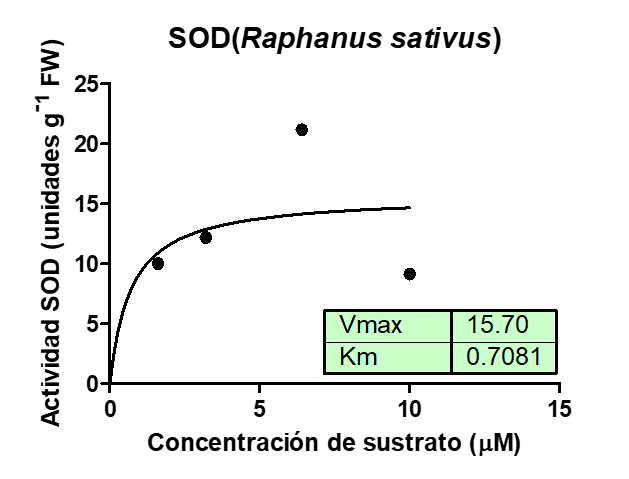
\includegraphics[scale=0.99]{Imagenes/SODacet}
	\caption{Cin\'etica enzim\'atica de Michaelis-Menten de la enzima SOD obtenida mediante el programa \textit{GraphPad Prism}. Se muestran los valores $K_ma$ y $V_{max}$ de SOD en plantas de \textit{R. sativus} que germinaron a partir de semillas que no fueron impregnadas previamente y no estaban sometidas a estr\'es. Se utiliz\'o el protocolo de extracci\'on con acetona \citep{baquero2005catalase}. Se analiza un único caso representativo (n=1) por lo que no se puede realizar análisis estadístico.}
	\label{SODacet}
\end{figure}

\pagebreak

\section{Enzima Catalasa (CAT).}

El extracto enzim\'atico fue preparado a partir de plantas que no estaban sometidas a estr\'es salino utilizando el protocolo de extracci\'on de \cite{liu2010exogenous} (primer dise\~no experimental, ep\'igrafe \ref{d1}). La concentraci\'on de prote\'inas fue de $10.82 \; \mu g/ \mu L$. Con los valores obtenidos se construy\'o la curva de cin\'etica enzim\'atica que se muestra en la figura \ref{cat}.\\

\begin{figure}[hbtp]
	\centering
	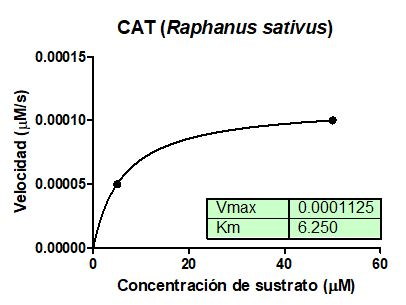
\includegraphics[scale=0.95]{Imagenes/CAT}
	\caption{Cin\'etica enzim\'atica Michaelis-Menten de la enzima CAT obtenida mediante el programa \textit{GraphPad Prism}. Se muestran los valores de $K_ma$ y $V_{max}$ de CAT en plantas de \textit{R. sativus} que germinaron a partir de semillas que no fueron impregnadas previamente y no estaban sometidas a estr\'es. La prote\'ina se extrajo mediante el protocolo de \cite{liu2010exogenous}. Se analiza un único caso representativo (n=1) por lo que no se puede realizar análisis estadístico.}
	\label{cat}
\end{figure}

\section{Enzima Polifenol Oxidasa (PPO).}\

Los extractos obtenidos mediante el segundo protocolo de extracci\'on enzim\'atica \citep{baquero2005catalase}, no mostraron resultados de la enzima PPO, no hubo variaci\'on en la DO, ni en la pendiente. 

\pagebreak

\subsection {PPO, primer dise\~no experimental: plantas no sometidas a estr\'es salino.}

El extracto enzim\'atico de plantas no sometidas a estr\'es salino, obtenido mediante el protocolo de extracci\'on propuesto por \cite{liu2010exogenous} (ep\'igrafe \ref{p1}), present\'o una concentraci\'on de $10.26 \;\mu g/ \mu L$ de prote\'ina. En la figura \ref{POd1} se muestra la cin\'etica enzim\'atica de Michaelis-Menten obtenida para las concentraciones de L-DOPA: $10\;mM$; $5\;mM$; $2.5\;mM$ y $1.125\;mM$.\\

\begin{figure}[hbtp]
	\centering
	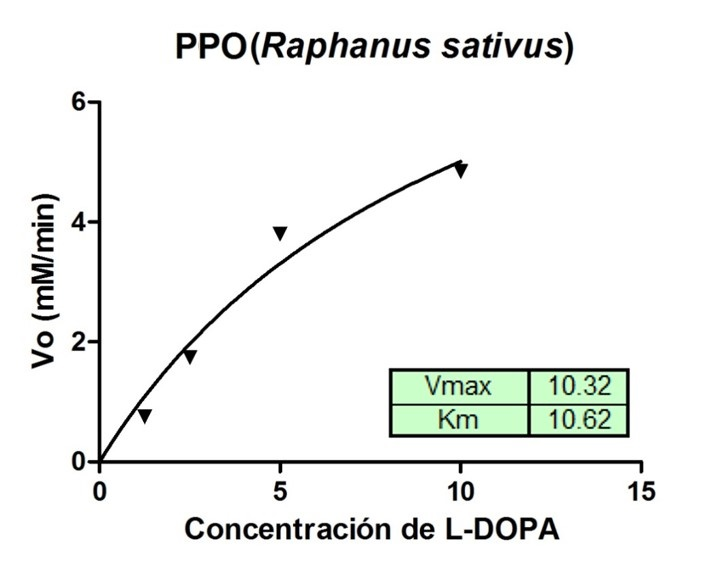
\includegraphics[scale=0.9]{Imagenes/POd1}
	\caption{Cin\'etica enzim\'atica Michaelis-Menten de la enzima PPO obtenida mediante el programa \textit{GraphPad Prism}. Se muestran los valores de $K_ma$ y $V_{max}$ de PPO en plantas de \textit{R. sativus} que germinaron a partir de semillas que no fueron impregnadas previamente y no estaban sometidas a estr\'es. El extracto se obtuvo mediante el protocolo de extracci\'on de \citep{liu2010exogenous}. Se analiza un único caso representativo (n=1) por lo que no se puede realizar análisis estadístico.}
	\label{POd1}
\end{figure} 

\pagebreak

\subsection {PPO, segundo dise\~no experimental: plantas sometidas a estr\'es salino.}

Seg\'un el procedimiento de \cite{liu2010exogenous}, con modificaciones, se obtuvieron dos extractos de plantas con tratamientos diferentes: control negativo ($10,13 \;\mu g/ \mu L$ de prote\'ina) y planta sometida a estr\'es salino ($9,78 \;\mu g/ \mu L$ de prote\'ina). Se muestra la cin\'etica enzim\'atica de Michaelis-Menten obtenida en la figura \ref{POkmVmax} para las concentraciones de L-DOPA: $7\;mM$; $5\;mM$ y $2.5\;mM$.\\

La comparaci\'on de los valores de $K_ma$ y $V_{max}$ obtenidos en cada uno de los extractos, se muestra en la figura \ref{PObarra}.\\

\medskip
\medskip
\medskip

\begin{figure}[h!!!!]
	\begin{subfigure}{.5\textwidth}
		\centering
		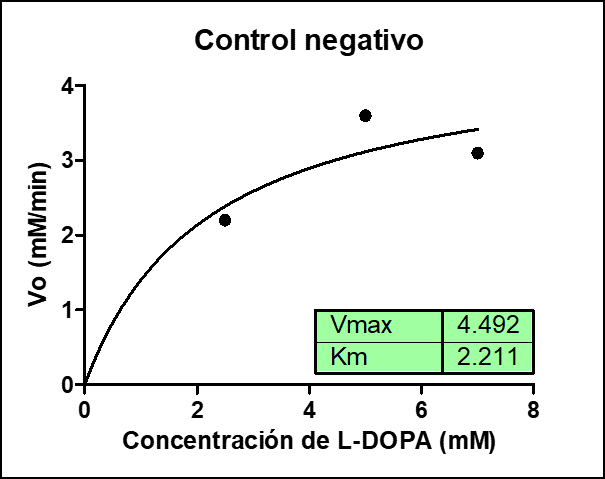
\includegraphics[width=.9\linewidth]{Imagenes/POnada}
		\caption{}
		\label{a}
	\end{subfigure}
	\begin{subfigure}{.5\textwidth}
		\centering
		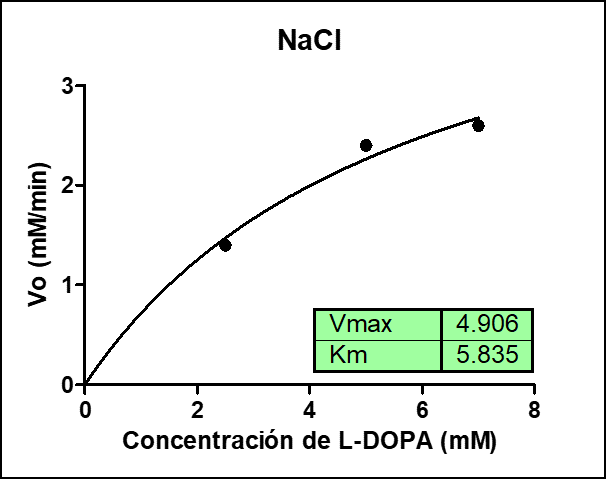
\includegraphics[width=.9\linewidth]{Imagenes/PONaCl}
		\caption{}
		\label{b}
	\end{subfigure}
	\caption{Cin\'etica enzim\'atica Michaelis-Menten de la enzima PPO obtenida mediante el programa \textit{GraphPad Prism}. Se muestran los valores de $K_ma$ y $V_{max}$ de PPO en plantas de \textit{R. sativus} que germinaron a partir de semillas impregnadas previamente con NaCl (sometidas a estr\'es salino) (b) y su control negativo (a). El extracto se obtuvo mediante el protocolo de extracci\'on de \citep{liu2010exogenous}. Se analiza un único caso representativo (n=1) por lo que no se puede realizar análisis estadístico.}
	\label{POkmVmax}
\end{figure}

\pagebreak

\begin{figure}[h!!!!]
	\begin{subfigure}{.5\textwidth}
		\centering
		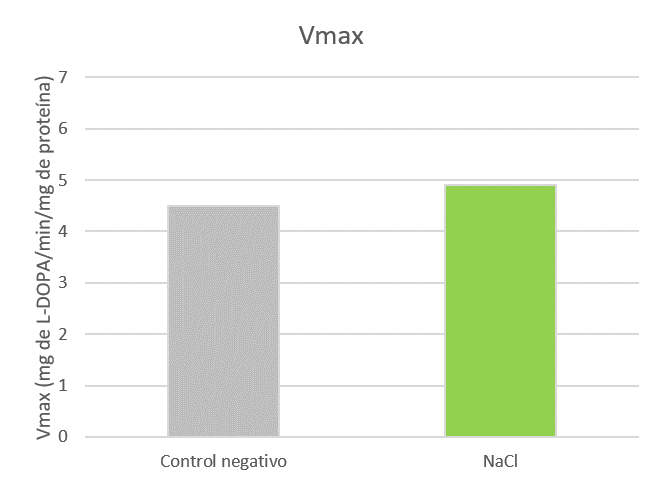
\includegraphics[width=.91\linewidth]{Imagenes/Vmax}
		\caption{}
		\label{1}
	\end{subfigure}
	\begin{subfigure}{.5\textwidth}
		\centering
		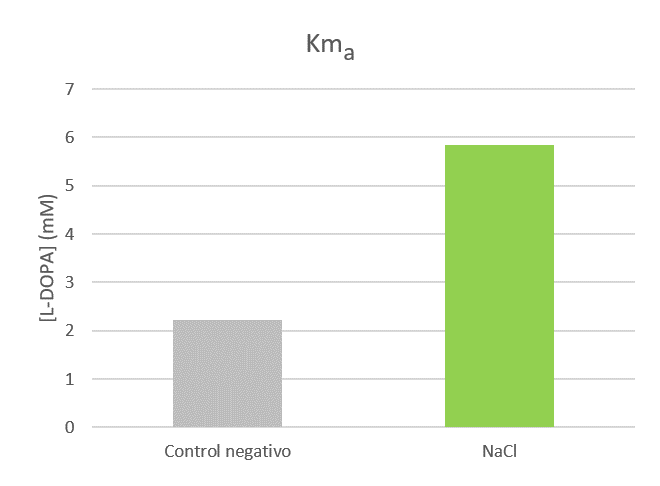
\includegraphics[width=.99\linewidth]{Imagenes/Km}
		\caption{}
		\label{2}
	\end{subfigure}
	\caption{Valores de $V_{max}$ (a) y $K_ma$ (b) de PPO obtenidos en plantas de \textit{R. sativus}, control negativo y sometidas a estr\'es por salinidad.}
	\label{PObarra}
\end{figure}

\medskip
\medskip

Como se observa en la figura \ref{PObarra} los valores de $V_{max}$ de las plantas control son muy similares a los obtenidos para las plantas sometidas a estr\'es por salinidad, pero si se observa un cambio en los valores de $K_ma$.

 
\chapter{Discusión}
\label{discus}

En el presente trabajo se lleva a cabo una propuesta preliminar de un protocolo para evaluar la eficiencia de brasinoesteroides sint\'eticos sobre la actividad de tres enzimas de defensa en plantas.  \\ 

La selecci\'on de \textit{Raphanus sativus} como modelo experimental se bas\'o en los numerosos trabajos cient\'ificos que detectan el incremento de la actividad de las enzimas de defensa, ante aplicaciones ex\'ogenas de BRs, aumentando as\'i la tolerancia de las plantas frente a distintos tipos de estr\'es. Por ejemplo, \cite{mahesh2013effect} utilizaron \textit{R. sativus} como modelo para analizar el efecto de dos an\'alogos de BRs (24-EpiBL y 28-HomoBL) y observaron el aumento de la actividad de enzimas antioxidantes, lo que disminuy\'o el efecto inhibitorio causado por estr\'es h\'idrico. \cite{anuradha2007effect} indican c\'omo al tratar plantas sometidas a estr\'es por Cadmio (Cd) con 24-EpiBL y 28-HomoBL aumenta la actividad de las enzimas antioxidantes SOD y CAT. La 24-EpiBL disminuy\'o los efectos de toxicidad del Cadmio (Cd) y el Mercurio (Hg), mediante la modulaci\'on de la actividad de enzimas antioxidantes, como SOD y CAT \citep{dhriti201424}; adem\'as, disminuy\'o el estr\'es oxidativo a trav\'es del incremento de la actividad de las enzimas de defensa, incluyendo PPO \citep{sharma2012effect}. \cite{ramakrishna2013preliminary} identificaron el aumento de la tolerancia en plantas de \textit{R. sativus} ante toxicidad por Zinc (Zn) al incrementar la actividad de enzimas antioxidantes, como resultado de la aplicaci\'on de 28-homoBL. Adem\'as, \cite{choudhary2012chromium} comprobaron que plantas de \textit{R. sativus} sometidas a estr\'es por Cobre (Cu), al ser tratadas con BRs ex\'ogenos pose\'ian mayor acumulaci\'on de enzimas antioxidantes.\\

En este trabajo se proponen dos dise\~nos experimentales que permiten la posterior evaluaci\'on de la actividad de las enzimas de defensa en plantas de \textit{R. sativus} y el efecto que pueden ejercer los an\'alogos sint\'eticos de BRs sobre la  actividad de las mismas. El protocolo propuesto permitir\'a determinar si existen diferencias en las respuestas generadas al aplicar los compuestos DI-31 y MH-5 en plantas sometidas a estr\'es salino, o no sometidas a este. \\

Existen diferentes v\'ias de aplicaci\'on ex\'ogena de BRs, entre las que se incluyen incubaci\'on de la semilla en el compuesto, tratamientos en las ra\'ices y aspersión foliar \citep{yusuf2019interplay}. Con el objetivo de evaluar si este elemento tiene influencia en el efecto de los tratamientos, se proponen dos v\'ias diferentes (aspersi\'on foliar e incubaci\'on de la semilla en el compuesto), lo que permitir\'a establecer cu\'al de estas es m\'as efectiva para desencadenar la respuesta de defensa. \\ 

%Entre los dise\~nos experimentales, el por qu\'e se decidi\'o probar un segundo m\'etodo en el que se sometieran las plantas a estr\'es previamente (ver el art\'iculo espec\'ifico por el cual vimos esto), al tener la consideraci\'on que probablemente las enzimas aumentar\'ian m\'as ante la inducci\'on de estr\'es por salinidad a pesar de que las ROS se encuentran tanto en plantas con estr\'es como en las que se encuentran en su estado basal. De todas formas el estr\'es por salinidad es una forma de retar la planta. \\


\section{Determinaci\'on de la cantidad de prote\'inas.}

El m\'etodo de cuantificaci\'on de prote\'inas Bradford descrito por primera vez por \cite{bradford1976rapid}, es una metodolog\'ia r\'apida, simple y certera para estimar la concentraci\'on de prote\'inas \citep{kruger2009bradford}. El colorante CBBG existe en dos formas de coloraci\'on diferente, rojo y azul. La forma roja es convertida a la azul al unirse el CBBG a la prote\'ina, lo que produce un incremento de absorci\'on de $465$ a $595\;nm$, que es monitoreado espectrofotom\'etricamente \citep{bradford1976rapid}. \\

El colorante se une más fácilmente a los residuos de arginina y lisina de las proteínas \citep{compton1985mechanism, congdon1993binding}. Esta especificidad puede conducir a variaciones en los resultados del ensayo frente a proteínas diferentes, siendo este el principal inconveniente del m\'etodo. El m\'etodo original de Bradford muestra gran variaci\'on en la respuesta a diferentes prote\'inas \citep{read1981minimization, friedenauer1989sensitivity, stoscheck1990increased}. Para solucionar este problema se han realizado numerosas variaciones a la metodolog\'ia, sin embargo, estos cambios generalmente resultan en un ensayo menos robusto, que a menudo es m\'as susceptible a interferencias. Consecuentemente, el método original ideado por \cite{bradford1976rapid} sigue siendo el m\'as conveniente y ampliamente  utilizado \citep{kruger2009bradford}. \\

Aunque los resultados del an\'alisis de varianza con los datos de concentración de proteínas fueron no significativos entre los distintos tiempos del experimento, a medida que pasa el tiempo disminuye la concentración de proteínas, por lo que los ensayos no se deben prolongar hasta cuatro d\'ias. \\

\section{Enzima Super\'oxido Dismutasa (SOD).}

%Comparaci\'on entre los resultados arrojados por cada uno de los protocolos de SOD, en este caso, se discute el mecanismo de la medici\'on mediante el reactivo pyrogallol y como la presencia de pigmentos puede haber influido en los resultados err\'oneos y como finalmente al extraer con acetona (explicar brevemente el m\'etodo con acetona como funciona) resuelve el problema de los pigmentos y los resultados en las curvas dan en el sentido correcto. \\

El m\'etodo de determinaci\'on de la actividad enzim\'atica de SOD, mediante la inhibici\'on de la autoxidaci\'on del Pyrogallol es uno de los m\'as utilizados, sin embargo, en la literatura se observan diferencias en las condiciones de ensayo empleadas. Por ejemplo, hay variaciones en la longitud de onda, la adici\'on o no de EDTA, el pH de la soluci\'on tamp\'on Tris-HCl, el solvente, el tiempo de ensayo y la temperatura, por lo que existen tambi\'en variaciones en los resultados obtenidos \citep{zhang2016optimization}. \\

El Pyrogallol se autoxida r\'apidamente en soluciones alcalinas, formando gran n\'umero de productos intermedios, cuya aparici\'on puede ser medida a $420\;nm$ (Fig. \ref{pyr}) \citep{marklund1974involvement}. La habilidad de SOD de inhibir la autoxidaci\'on del Pyrogallol (al generar super\'oxido) ha sido empleada de forma exitosa para la cuantificaci\'on de esta enzima. El Pyrogallol es un buen reductor de hierro (Fe) y el hierro reducido se puede autoxidar r\'apidamente generando radicales hidroxilo, lo que produce interferencias en el ensayo. La adici\'on de agentes quelantes como DETAPAC y EDTA en la mezcla del ensayo, elimina la posibilidad de interferencias de los iones $Fe^{2+}$, $Cu^{2+}$ y $Mn^{2+}$ \citep{pandey2014oxidative}, aunque pueden existir interferencias peque\~nas de $Fe^{2+}$ \citep{misra1972role, marklund1974involvement}. \\

\begin{figure}[hbtp]
	\centering
	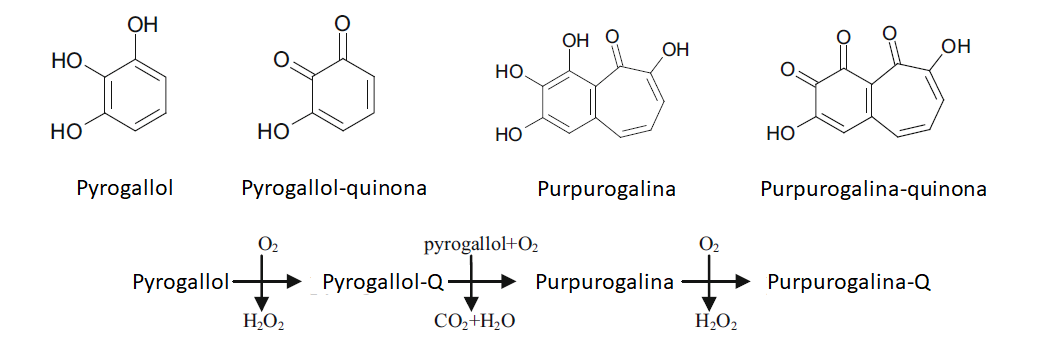
\includegraphics[scale=0.6]{Imagenes/pyr}
	\caption{Productos y secuencia de reacci\'on del Pyrogallol. Modificado de \cite{ramasarma2015new}.}
	\label{pyr}
\end{figure}

La velocidad de autoxidaci\'on del Pyrogallol depende fuertemente de su concentraci\'on y del pH. Adem\'as, existen otras mol\'eculas redox de bajo peso molecular que pueden reaccionar directamente con el diox\'igeno, aumentando la velocidad de autoxidaci\'on del Pyrogallol \citep{gao1998mechanism}. \\



%Cuando el radical superóxido se acumula y produce la autooxidación del pirogalol da lugar a la formación de purpurogalina, un compuesto amarillo-marrón con un pico máximo de absorbancia de luz a 420 nm y coeficiente de extinción molar 2640 M?¹cm?¹. Cuando hay SOD presente en el medio, la enzima compite con el pirogalol por el radical superóxido, inhibiéndose la reacción de autooxidación, lo que implica menor formación de purpurogalina. La formación de purpurogalina es susceptible de ser medida espectrofotométricamente en el tiempo, con lo que se puede aprovechar el fenómeno para cuantificar la actividad SOD de una muestra problema midiendo la inhibición de la autooxidación del pirogalol respecto de un control

En las tablas \ref{24hSOD}, \ref{48hSOD} y \ref{96hSOD} se observa que la velocidad de autoxidaci\'on del Pyrogallol en la soluci\'on tamp\'on,  siempre es menor o igual que la velocidad para los extractos, por lo que aparentemente no se produce inhibici\'on de la autoxidaci\'on del Pyrogallol, que te\'oricamente deber\'ia existir producto de la actividad de SOD. Esto se puede deber a interferencias de algunos de los componentes del extracto que determinan una mayor autoxidación de la que la enzima puede contrarrestar. \\

La adición de EDTA en mayor proporción no cambi\'o el  resultado obtenido, luego la presencia de algún catión divalente no autoxidaba el sustrato. Por tanto, 1mM de EDTA es suficiente para impedir la influencia de estos cationes, lo que se corresponde con lo indicado por \cite{marklund1974involvement}. \\

El protocolo de extracción con acetona \citep{baquero2005catalase} eliminaría las interferencias de pigmentos, por lo que se decidi\'o extraer la enzima mediante este protocolo y evaluar la actividad de SOD en este extracto.\\

La técnica de extracción enzim\'atica con acetona  empleada en este trabajo se basó en reportes previos, en los que se obtenía una buena eficiencia en la extracción de proteína y en la actividad enzimática \citep{sala1999catalase,  narvaez2002evaluacion, camelo2004polifenoloxidasa}. Los polvos de acetona permiten que el extracto presente una alta actividad con una mayor estabilidad, además de evitar la inactivación enzimática durante la extracción, porque con la acetona se retiran los fenoles, $\beta$-carotenos y ácidos orgánicos del extracto, disminuyendo así la reacción de las enzimas con estos compuestos \citep{baquero2005catalase}. Otros art\'iculos, por ejemplo \cite{lopez2014actividad} tambi\'en emplean protocolos de extracci\'on similares. \\

Dado los resultados obtenidos en el presente trabajo, es probable que la causa del incremento de la autoxidaci\'on del Pyrogallol sea la presencia de sustancias como fenoles, $\beta$-carotenos y ácidos orgánicos. Los extractos obtenidos mediante el protocolo de extracci\'on de \cite{baquero2005catalase} (con modificaciones) presentaron actividad de la enzima SOD, aunque por este protocolo hay una p\'erdida importante de prote\'inas.\\


\section{Enzima Catalasa (CAT)}

%En el caso de CAT TODAS las consideraciones que hay que tener encuenta para medir esta enzima. En los art\'iculos que est\'an en la literatura solo miden 2 puntos y asumen que la enzima tiene un comportamiento lineal, pero realmente en niguno de los art\'iculos miden m\'as de dos puntos, solo en el tiempo inicial y en el final y se restan ambos puntos. No observan la linealidad de la enzima. 

La metodolog\'ia m\'as utilizada para medir la actividad de la enzima CAT es la medici\'on espectrofotom\'etrica del cambio de absorbancia a $240\;nm$ ante altos niveles de per\'oxido de hidr\'ogeno (mayores o iguales a $30\;mM$). Los altos niveles de per\'oxido de hidr\'ogeno llevan inmediatamente a la inhibici\'on de la enzima CAT, alterando la estructura de su centro activo. Existe la necesidad de un m\'etodo para evaluar continuamente la baja actividad de la enzima CAT frente a un fondo de alto nivel de absorbancia que se produce debido a que muchos constituyentes celulares, como \'acidos nucleicos y prote\'inas exhiben una intensa absorci\'on a $240\;nm$ \citep{hadwan2018simple}.\\

La cin\'etica de la CAT no sigue un patr\'on usual. Primeramente, no es posible saturar la enzima con sustrato dentro del intervalo de concentraciones menores a $5\;M$ de per\'oxido de hidr\'ogeno. Por otra parte, a concentraciones mayores de $0.1\;M$ ocurre una r\'apida inactivaci\'on de la enzima. En consecuencia, la determinaci\'on de la actividad a concentraciones saturantes, no es posibles. En contraste a las reacciones que se desarrollan a concentraciones saturantes de sustrato, la descomposici\'on enzim\'atica del per\'oxido de hidr\'ogeno es una reacci\'on de primer orden, por lo que la tasa de reacci\'on es proporcional a la cantidad de per\'oxido de hidr\'ogeno presente. Para evitar una r\'apida disminuci\'on en la tasa inicial de la reacci\'on, esta se debe llevar a cabo con concentraciones de $H_2O_2$ bajas (alrededor de $0.01\;M$) \citep{aebi198413}.\\

Este trabajo condujo a la identificaci\'on de posibles causas de errores en la medici\'on de la CAT. Por ejemplo, el extracto enzim\'atico debe ser adicionado y al instante realizar la medici\'on espectrofotom\'etrica, que debe realizarse espec\'ificamente en cubetas de cuarzo. El pH debe ser controlado y es necesario evitar que el extracto enzim\'atico experimente procesos de congelaci\'on-descongelaci\'on. Adem\'as se debe comprobar que no existan burbujas en las paredes de la cubeta. \\ 

%Art\'iculos a citar donde solo miden 2 puntos a 15 y 180 segundos:
%
%\citep{lopez2014actividad}

\section{Enzima Polifenol Oxidasa (PPO).}

%- En el caso de PPO ver el logro de realizar este protocolo en placas, pues el extracto es limitado. Ver que con el extracto de acetona no funciona. Ver lo del art\'iculo del dise\~no 2 que explica los resultados que tenemos.\\ 

El compuesto L-DOPA posee un gran potencial como sustrato modelo para estudios de la degradaci\'on enzim\'atica de compuestos fen\'olicos. En presencia de la enzima PPO es convertido r\'apidamente a 2-carboxi 2,3-dihidroindol 5,6-quinona, que puede ser medido espectrofotom\'etricamente a $475\;nm$ \citep{pind1994enzymic}.\\

La PPO es una de las enzimas responsables de la oxidaci\'on de compuestos fen\'olicos \citep{sheen1969studies} y la disminuci\'on de su actividad puede inducir una acumulaci\'on de fenoles totales \citep{das1992sodium}. \cite{muthukumarasamy2000enhancement} comprobaron que la actividad enzim\'atica de PPO en plantas, disminuye ante e estr\'es por salinidad, lo que puede llevar al da\~no oxidativo. \\

Al comparar los valores de $K_ma$ de las plantas que germinaron a partir de semillas que no fueron incubadas en agua previo a su siembra (Fig. \ref{POd1}) con los valores de semillas que si fueron incubadas en agua (Fig. \ref{a}), podemos observar como la incubaci\'on afecta positivamente el valor de este par\'ametro, lo que coincide con los informes encontrados en la literatura \citep{burgass1984evidence, bradford1986manipulation, taylor1998seed, mcdonald2000seed}. En el caso de $V_{max}$ las plantas de semillas que no fueron incubadas en agua previo a su siembra (Fig. \ref{POd1}), mostraron un valor mayor de este par\'ametro que las plantas incubadas en agua y las sometidas a estr\'es salino (Fig. \ref{POkmVmax}). No se puede llegar a conclusiones reales a partir de los valores obtenidos, pues se trata de ensayos puntuales, en los que no se pueden realizar an\'alisis estad\'isticos.\\


En el trabajo realizado la variaci\'on entre los valores de $V_{max}$ de plantas sometidas a estr\'es por salinidad y su control negativo fue peque\~na, como se puede observar en la figura \ref{1}.\\

Por su parte los valores obtenidos de $K_ma$ mostraron una mayor variaci\'on. En este caso, como se muestra en la figura \ref{2}, los extractos obtenidos a partir de plantas de \textit{R. sativus} sometidas a estr\'es presentaron un valor de $K_ma$ mayor, con respecto al control negativo, lo que pudiese indicar aumentos de la afinidad de la enzima por el sustrato en respuesta al estr\'es salino.\\

Al medir la actividad enzim\'atica de PPO en extractos realizados seg\'un la metodolog\'ia de extracci\'on de \cite{baquero2005catalase}, no se observ\'o actividad de la enzima. En este sentido, se recomienda utilizar otra soluci\'on tamp\'on para diluir el precipitado proteico formado en el ensayo y la utilizaci\'on de un sustrato diferente, por ejemplo: catecol \citep{martinez2013actividad}.





\chapter{Conclusiones}
%===================================================================================
% Chapter: Conclusion
%===================================================================================
%\chapter*{\Huge Conclusiones}\label{chapter:conclusion}
%\addcontentsline{toc}{chapter}{Conclusiones y Recomendaciones}
%===================================================================================


\begin{enumerate}
\item Se determin\'o la metodolog\'ia propuesta por \cite{baquero2005catalase} (con modificaciones) para la obtenci\'on de extractos crudos donde se pueda evaluar la actividad de la enzima SOD. La metodolog\'ia propuesta por \cite{liu2010exogenous} (con modificaciones) fue seleccionada para la obtenci\'on de extractos crudos, donde se pueden evaluar las enzimas CAT y PPO.\\
\item Se estableci\'o el ensayo de \cite{ma2009spectroscopic}, con modificaciones, para medir los par\'ametros cin\'eticos de la enzima SOD, el protocolo de \citep{chance1955136}, con modificaciones para el an\'alisis de la enzima CAT y el ensayo de \cite{baquero2005catalase}, con modificaciones para la determinaci\'on de los par\'ametros de la enzima PPO.

\end{enumerate}




\chapter{Recomendaciones}


\begin{enumerate}
\item Determinar la actividad de las enzimas SOD, CAT y PPO siguiendo los protocolos descritos, para evaluar el efecto de los an\'alogos sint\'eticos de BRs.
\end{enumerate}


















\backmatter

\renewcommand{\bibname}{Literatura Citada}
\bibliographystyle{my-bath}
\bibliography{Bibliography}

\renewcommand{\figurename}{Figura}


%















%===================================================================================
% Chapter: Anexos
%===================================================================================
\chapter*{\Huge Anexos}\label{chapter:anexos}
\addcontentsline{toc}{chapter}{Anexos}
%===================================================================================


\setcounter{figure}{0}
\section *{Anexo 1} \label{ane1}
 \begin{center}
	{\Large Prueba de normalidad Anderson-Darling}
\end{center}
\medskip
\medskip
\medskip
\medskip
\begin{figure}[h]
\begin{subfigure}{.5\textwidth}
	\centering
	\includegraphics[width=.85\linewidth]{Imagenes/distralfa1.jpg}
	\caption{}
	\label{distralfa}
\end{subfigure}
\begin{subfigure}{.5\textwidth}
	\centering
	\includegraphics[width=.85\linewidth]{Imagenes/distrbeta1.jpg}
	\caption{}
	\label{distrbeta}
\end{subfigure}
\par\bigskip
\begin{subfigure}{.5\textwidth}
	\centering
	\includegraphics[width=.85\linewidth]{Imagenes/distrmfo1.jpg}
	\caption{}
	\label{distrmfo}
\end{subfigure}
\begin{subfigure}{.5\textwidth}
	\centering
	\includegraphics[width=.85\linewidth]{Imagenes/distrgst1.jpg}
	\caption{}
	\label{distrgst}
\end{subfigure}
\caption{Distribución de los valores de actividad enzimática (AE) de las muestras de la cepa de referencia susceptible Fraga para cada enzima de actividad metabólica. Prueba de normalidad Anderson-Darling. (a) $\alpha$ esterasas $R^{2}=0,9625$, (b) $\beta$ esterasas $R^{2}=0,9761$, (c) MFO $R^{2}=0,9375$ y (d) GST $R^{2}=0,9817$.}
\label{distribucion}
\end{figure}

\begin{figure}[h]
\begin{subfigure}{.5\textwidth}
	\centering
	\includegraphics[width=.85\linewidth]{Imagenes/normalzooalfa.jpg}
	\caption{}
	\label{distralfa}
\end{subfigure}
\begin{subfigure}{.5\textwidth}
	\centering
	\includegraphics[width=.85\linewidth]{Imagenes/normalzoobeta.jpg}
	\caption{}
	\label{distrbeta}
\end{subfigure}
\par\bigskip
\begin{subfigure}{.5\textwidth}
	\centering
	\includegraphics[width=.85\linewidth]{Imagenes/normalzoomfo.jpg}
	\caption{}
	\label{distrmfo}
\end{subfigure}
\begin{subfigure}{.5\textwidth}
	\centering
	\includegraphics[width=.85\linewidth]{Imagenes/normalzoogst.jpg}
	\caption{}
	\label{distrgst}
\end{subfigure}
\caption{Distribución de los valores de actividad enzimática (AE) de las muestras de la cepa Zoológico 26 para cada enzima de actividad metabólica. Prueba de normalidad Anderson-Darling. (a) $\alpha$ esterasas $R^{2}=0,9182$, (b) $\beta$ esterasas $R^{2}=0,9695$, (c) MFO $R^{2}=0,9775$ y (d) GST $R^{2}=0,9301$.}
\label{distribucion}
\end{figure}



\begin{figure}[h]
\begin{subfigure}{.5\textwidth}
	\centering
	\includegraphics[width=.85\linewidth]{Imagenes/normalmulgobaalfa.jpg}
	\caption{}
	\label{distralfa}
\end{subfigure}
\begin{subfigure}{.5\textwidth}
	\centering
	\includegraphics[width=.85\linewidth]{Imagenes/normalmulgobabeta.jpg}
	\caption{}
	\label{distrbeta}
\end{subfigure}
\par\bigskip
\begin{subfigure}{.5\textwidth}
	\centering
	\includegraphics[width=.85\linewidth]{Imagenes/normalmulgobamfo.jpg}
	\caption{}
	\label{distrmfo}
\end{subfigure}
\begin{subfigure}{.5\textwidth}
	\centering
	\includegraphics[width=.85\linewidth]{Imagenes/normalmulgobagst.jpg}
	\caption{}
	\label{distrgst}
\end{subfigure}
\caption{Distribución de los valores de actividad enzimática (AE) de las muestras de la cepa Mulgoba para cada enzima de actividad metabólica. Prueba de normalidad Anderson-Darling. (a) $\alpha$ esterasas $R^{2}=0,9645$, (b) $\beta$ esterasas $R^{2}=0,9492$, (c) MFO $R^{2}=0,9037$ y (d) GST $R^{2}=0,9672$.}
\label{distribucion}
\end{figure}
\clearpage

\setcounter{figure}{0}
\section *{Anexo 2} \label{ane2}
\begin{center}
	{\Large Porcentaje de actividad enzimática ($P_{99}$)}
\end{center}
\medskip
\medskip
\medskip
\medskip
\begin{figure}[h]
\begin{subfigure}{.5\textwidth} 
	\centering
	\includegraphics[width=\linewidth]{Imagenes/alfa99.jpg}
	\caption{}
	\label{alfa99}
\end{subfigure}
\begin{subfigure}{.5\textwidth}
	\centering
	\includegraphics[width=\linewidth]{Imagenes/beta99.jpg}
	\caption{}
	\label{beta99}
\end{subfigure}
\par\bigskip
\begin{subfigure}{.5\textwidth}
	\centering
	\includegraphics[width=\linewidth]{Imagenes/mfo99.jpg}
	\caption{}
	\label{mfo99}
\end{subfigure}
\begin{subfigure}{.5\textwidth}
	\centering
	\includegraphics[width=\linewidth]{Imagenes/gst99.jpg}
	\caption{}
	\label{gst99}
\end{subfigure}
\caption{Valores medios de actividad enzimática (AE) de (a) $\alpha$ esterasas, (b) $\beta$ esterasas, (c) MFO  y (d) GST para las cepas Zoológico 26,  Mulgoba y la cepa de referencia susceptible Fraga. La línea horizontal de color negro indica el valor de corte establecido por la cepa Fraga (valor del percentil 99 ($P_{99}$).)}
\label{figura:99}
\end{figure}
\clearpage

\setcounter{figure}{0}
\section *{Anexo 3} \label{ane3}
\begin{center}
	{\Large Porcentaje de actividad enzimática ($P_{95}$)}
\end{center}
\medskip
\medskip
\medskip
\medskip
\begin{figure}[h]
\begin{subfigure}{.5\textwidth}
	\centering
	\includegraphics[width=\linewidth]{Imagenes/alfa95.jpg}
	\caption{}
	\label{alfa95}
\end{subfigure}
\begin{subfigure}{.5\textwidth}
	\centering
	\includegraphics[width=\linewidth]{Imagenes/beta95.jpg}
	\caption{}
	\label{beta95}
\end{subfigure}
\par\bigskip
\begin{subfigure}{.5\textwidth}
	\centering
	\includegraphics[width=\linewidth]{Imagenes/mfo95.jpg}
	\caption{}
	\label{mfo95}
\end{subfigure}
\begin{subfigure}{.5\textwidth}
	\centering
	\includegraphics[width=\linewidth]{Imagenes/gst95.jpg}
	\caption{}
	\label{gst95}
\end{subfigure}
\caption{Valores medios de actividad enzimática (AE) de (a) $\alpha$ esterasas, (b) $\beta$ esterasas, (c) MFO  y (d) GST para las cepas Zoológico 26,  Mulgoba y la cepa de referencia susceptible Fraga. La línea horizontal de color negro indica el valor de corte establecido por la cepa Fraga (valor del percentil 95 ($P_{95}$).)}
\label{figura:95}
\end{figure}

\end{document}